\chapter{Decision Problems}

\section{Games Against Nature}


% also we need a section on using backward induction to solve
% decisions over time. relate it to DP.

\section{Games Against an Opponent}

% this will be the last portion of this section, where we bring together
% several concepts. Need to re-write this section: change the context
% of the problem and explain the methodology.
\emph{Nature as an adversary: a two-person zero-sum game.}
Merrill has a concession stand at Target Field for the sale of
sunglasses and umbrellas. This entrepreneur likes to make sales
regardless of the weather.  When it rains can sell about 500
umbrellas.  On a sunny day he can sell about 100 umbrellas and about
1000 sunglasses. Umbrellas cost him 50 cents and sell for \$1.
Sunglasses cost him 20 cents each and sell for 50 cents. Merrill is
willing to invest \$250 in the concession stand business.  All unsold
items represent a loss; there is no salvage value. 

Formulate Merrill's problem as a two-person zero--sum game. Merrill is
the row player and Nature is the column player. Merrill's strategy set
is \{buy inventory for rain, buy inventory for sun\}. Nature's strategy
set is \{rain, sun\}. The payoff entries represent the profit/loss.
Find an equilibrium strategy for Merrill. That is
to say, Merrill treats Nature as a strategic opponent and wants to
find an optimal inventory strategy that will yield a maximum expected
profit \emph{regardless} of the weather.

Would Merrill necessarily need to invest all \$250 into buying inventory
exclusively for rain or sun? In other words, does it seem possible that
Merrill could truly mix his two pure strategies and invest a portion
of the \$250 into each? The game is

\begingroup
\setlength{\tabcolsep}{9pt}
\renewcommand*{\arraystretch}{2}
\begin{tabularx}{4in}{YYYY}
& & \multicolumn{2}{c}{Nature} \\
& & Rain & Sun \\ \cline{3-4}
\multirow{2}{.5in}{Merrill} & \gtcol{Rain} & \gtcol{250} & \gtcol{-150} \\ \cline{3-4}
& \gtcol{Sun} & \gtcol{-150} & \gtcol{350} \\ \cline{3-4}
\end{tabularx}
\endgroup
\vspace{.1in}

The best strategy for Merrill is to mix buying for rain and buying
for sun in the ratio 5 to 4. These are the odds. To compute 
Merrill's expected profit (i.e. the value of the game) we use
Merrill's  equilibrium strategy against either of Nature's
pure strategies. Here is the payoff for Merrill against
Nature's strategy of Rain.

\[ \frac{5 \times (250) + 4 \times (-150)}{9} = \$72.22 \]

Merrill could play the odds and choose a pure strategy, but 
note that in this game it is possible for Merrill to physically
mix the strategies. He could invest 5/9 of his \$250 in
rainy--day inventory and invest 4/9 in sunny--day inventory.
So he buys
\[ \frac{5}{9} \left(500 \times .50\right) + \frac{4}{9} \left(100 \times .50\right) = \$161.11 \]
worth of umbrellas and
\[ \frac{4}{9} \left(1000 \times .20\right) = \$88.89 \]
worth of sunglasses so that he enjoys a steady profit of \$72.22.

\section{Utility Theory}
The payoffs in the decision problems that we have discussed have been
either monetary values or ``utilities''. So far, we haven't said much
about them.  In this section, we provide a bit more detail about the
payoff values in a decision problem.  The purpose of utility theory is
to have a convenient way to represent personal preferences over
outcomes, and by \emph{convenient} we mean numerical~\cite{luce:1957},
\cite{peterson:2009},\cite{resnik:1987}. Why is utility
important? How can utility for outcomes be more useful than simply
stating our preferences?

\begin{quote} % need to find the source ... luce and raiffa i think
Utilities are more
useful than a list of preferences for the same reason that Arabic
numerals are more useful than Roman numerals; they are better at
facilitating the transfer of information. 
\end{quote} 

It is important to note that we are not trying to explain why a
decision-maker has certain preferences over outcomes. We are just
trying to represent the preferences numerically. It turns out that
utilities are measured on an interval scale, as opposed to a ratio
scale. We cannot add, subtract, multiply, or divide utilities as we do
with measurements such as length, weight and speed, and we cannot
compare the utilities among different persons (unless they have the
same utility function).  Nevertheless, utilities capture attitudes
toward risk and utility theory is fundamental to understanding
decision problems.
\vspace{.2in} 

\begin{wrapfigure}{r}{.33\textwidth}
\centering
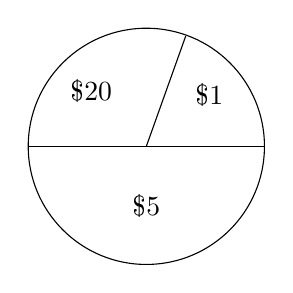
\begin{tikzpicture}
\draw (-1.5,0) -- (1.5,0);
\draw (0,0) -- (.5,1.4);
\draw (0,0) circle (1.5cm);
\draw (0,-.75) node {\$5};
\draw (-.7,.7) node {\$20};
\draw (.8,.65) node {\$1};
\end{tikzpicture}
\end{wrapfigure}

Sometimes taking a simple expected value makes sense.  Consider a
gamble in which one of three outcomes will occur. The outcomes are
worth \$1, \$5, and \$20 and the probabilities of the outcomes are .2,
.5, and .3, respectively. For example, a wheel is spun and the
probability of winning an amount corresponds to the area on the wheel.
The expected monetary value (EMV) of the gamble is
\[ \$1 \times .2 + \$5 \times .5 + \$20 \times .3 = \$8.70 \]

However, there exist situations where EMV is not an appropriate
indicator of ``fair value''. Consider another gamble in which a fair
coin is tossed until the first head appears. The gambler receives
$\$2^n$ where $n$ is the number of the tosses required until the first
instance of heads appears. So there will be $n-1$ tails followed by
heads. The probability of the first instance of heads occurring on
toss $n$ is $(1/2)^n$ and the EMV of the gamble is
\[
  2\left(\frac{1}{2}\right) + 4\left(\frac{1}{4}\right) + 8\left(\frac{1}{8}\right) +
  16\left(\frac{1}{16}\right) + \ldots = \infty.
\]
Few people (perhaps no one) would pay any amount to participate in the
gamble.  This is the St. Petersburg paradox stated by Bernoulli. To
resolve the paradox, he said that the monetary value is not as
important as the ``intrinsic worth'' of the money. For many people, an
increase in the amount of money has increasing worth, but at a
decreasing rate. Given an amount of money $m$, the logarithmic
function captures the basic relationship between $m$ and its
``intrinsic worth'' (see Figure~\vref{fig:diminishing}).

\begin{figure}
\centering
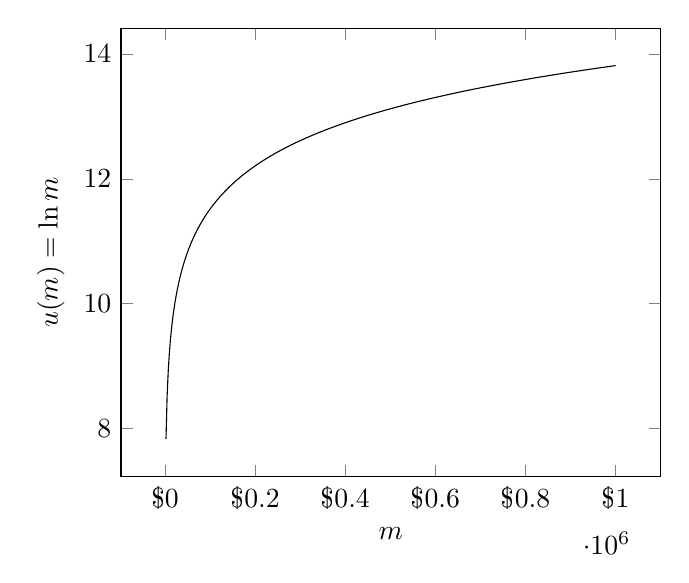
\begin{tikzpicture}
\begin{axis}[
    xlabel={$m$},
    ylabel={$u(m) = \ln m$},
    xticklabel={\$$\pgfmathprintnumber{\tick}$},
    %title={}
  ]
  \addplot[domain=0:1000000,samples=400] {ln(x)};
\end{axis}
\end{tikzpicture}
\caption{The diminishing rate of the value of money.}
\label{fig:diminishing}
\end{figure}

However, there are many functions with this basic shape and they
differ from person to person. How can the value (or utility) of money
be specified for an individual? Also, expected value is commonly
associated with value over the long run. What about a one-time
gamble? Von Neumann and Morgenstern (VnM~\cite{vonneumann:1953})
showed how to construst a utility that
represents a decision-maker's preferences (numerically) among gambles. Note that if
we were only concerned with choices among basic (certain) alternatives
then the decision-maker would simply rank the alternatives in an
ordinal manner. But we are concerned with decision-making under
risk. When we allow gambles, and ask a person to express preferences
over pairs of gambles (where the gambles are over basic alternatives)
then VnM showed how to associate utilities to the basic alternatives
in such a way that 
\begin{inparaenum}[1)] 
\item the utility for an alternative is measured by
the risk one is willing to take to receive it~\cite{savage:1972}, and
\item if decisions are made based on expected utility, then the
decision--maker is acting in agreement with her preferences.
\end{inparaenum}
Of course, the decision-maker's preferences must have some amount of
consistency. In other words, preferences must obey some rules that we
will state later.

Here is the basic idea for the construction of a utility function.
Suppose that among three different bands, Alice prefers
Smashing Pumpkins to Yo La Tengo, and she prefers Yo La Tengo to Wilco.
Now any three numbers that decrease in magnitude will capture
the ordinal preferences. But we are allowing gambles so that
we can capture Alice's attitude toward risk. We allow Alice
to choose between two alternatives 
\begin{inparaenum}[1)]
\item seeing Yo La Tengo for sure, or 
\item a gamble where she sees Smashing Pumpkins with probability
$p$ or Wilco with probability $1-p$. 
\end{inparaenum}
If $p$ is very close to one then Alice will choose the gamble. But if we
decrease $p$, then at \emph{some} point Alice will prefer the certain
alternative of seeing Yo La Tengo. We ask Alice for the value of
$p$ at which she is indifferent between the certain alternative and
the gamble. Suppose Alice indicates
$p=2/3$. Now, arbitrarily associate the value 1 with Smashing Pumpkins
and associate the value 0 with Wilco. Then it seems natural to
associate the value 2/3 with Yo La Tengo. Note that the value of Yo La
Tengo equals the expected value of the gamble.
\[ \frac{2}{3} = 1\left(\frac{2}{3}\right) +
  0\left(\frac{1}{3}\right) \] Instead of using (1, 2/3, 0) we could
use \emph{any} three numbers $a+c,~(2/3)a+c,~c$, where $a$ and
$c$ are constants and
$a>0$, and not alter the preferences (including the preference over the
certain outcome and the gamble).

Perhaps the most troublesome aspect of constructing utilities in this
way is the natural inclination to think about the utility values in
terms of ratios. You should avoid doing this.  For example, it is
\emph{not} correct to say that Alice prefers seeing Yo La Tengo to
seeing Wilco twice as much as she prefers seeing Smashing Pumpkins to
seeing Yo La Tengo. No! The number 2/3 reflects Alice's attitude
toward gambling, not her attitude toward the two intervals. A commonly
used example~\cite{luce:1957} to illustrate this fact is the
following. Suppose you like taking chances. You are
indifferent between 1) receiving \$9 for sure, or 2) participating in
a gamble that results in equal chances of receiving either \$10 or
nothing. Your utilities for the three amounts \$10, \$9 and \$0 are 1,
1/2, and 0, respectively. It's not that you have equal preferences
for going from \$0 to \$9 and going from \$9 to \$10. No. You simply
like taking chances.

Another common mistake is to say that Alice prefers Smashing Pumpkins
to Yo La Tengo because Smashing Pumpkins has higher utility. No!
Alice's preferences (and your preferences) among basic alternatives
and lotteries come first. A decision-maker knows her preferences. The
point is that if Alice can state her preferences, then we can
construct a numerical characterization of them. That is to say, we can
associate a value (i.e. a number) to something that is inherently
non-numeric.  The expected utility theorem is a representation
theorem.

\label{rules-of-consistency}
Now for the rules of consistency. Let $L(p,x,y)$ represent a gamble
(also called a lottery) in which you receive outcome $x$ with
probability $p$ or you receive outcome $y$ with probability
$(1-p)$. Also, let $x \succ y$ indicate that outcome $x$ is preferred
to outcome $y$, and let $x \sim y$ indicate indifference between the
outcomes $x$ and $y$. A decision-maker's preferences must satisfy the
following rules. (Note that the rules don't seem too objectionable).
\begin{enumerate}
\item $x \succ y$ or $y \succ x$ or $x \sim y$. (completeness)
\item if $x \succ y$ and $y \succ z$ then $x \succ z$. (transitivity)
\item $L\left(p,L(q,x,y),L(r,x,y)\right) \sim L(s,x,y)$ where $s=pq+(1-p)r$. (no fun in gambling)
\item given $x \succ y \succ z$, there is some lottery $L(p,x,z) \sim y$. (continuity)
\item if two lotteries are identical except for the first prize, then the
  lottery with the better first prize is preferred. (better prizes condition)
\item if two lotteries have the same alternatives as prizes, then the
  lottery that assigns higher probability of winning the best prize is
  preferred. (better chances condition)
\end{enumerate}
If you can state your preferences according to the above rules,
then an \emph{interval} utility function $u()$ can be constructed
in such a way that
\begin{enumerate}[i)]
\item $u(x) \succ u(y) \iff x \succ y$ \label{eu1}
\item $u(x) = u(y) \iff x \sim y$ \label{eu2}
\item $u\left(L(p,x,y)\right) = pu(x) + (1-p)u(y)$ 
(expected utility property) \label{eu3}
\item if $u'()$ is a positive linear transformation of $u()$ then
  $u'()$ also satisfies \ref{eu1}, \ref{eu2}, and \ref{eu3}. \label{eu4}
\end{enumerate}
Items \ref{eu1} through \ref{eu4} constitute the Expected Utility
Theorem.  When working through exercises, perhaps the most useful item is
item \ref{eu3}, the expected utility property. It states that the utility
of a lottery is equal to its expected utility. Do \emph{not} confuse
expected utility with the utility of the expected value, which is not
of interest.

\emph{Retirement and risk}.  This example is inspired from the
discussion on utility in Chernoff and Moses~\cite{chernoff:1959}.
Alice currently has \$\num{400000} in her individual retirement
account (IRA). Of course, it is always better to have more money for
retirement, but Alice is not super-greedy; she wants to have enough
money to pay bills and take a few backpacking trips each year.  Her
utility for an amount of money $m$ in the range \$0 to \$1 million is
given by the following function and is shown in
Figure~\vref{fig:retirement}.

\[
u(m) = \frac{10}{1+e^{-(\frac{m}{\num{500000}}-5)}}
\]

\begin{figure}
\centering
\begin{tikzpicture}
\begin{axis}[
    xlabel={$m$},
    ylabel={$u(m)$},
    xticklabel={\$$\pgfmathprintnumber{\tick}$},
    %title={Utility function for the retirement funds}
  ]
  %\addplot[domain=0:1000000,samples=1000] {10 / (1 + exp(-(x/500000 - 5)))};
  % tikz was plottting the function incorrectly, so for now i am resorting
  % to coordinates.
  \addplot[color=black,mark=none]
  coordinates {
(0,0.0669)(1000,0.0676)(2000,0.0683)(3000,0.069)(4000,0.0696)
(5000,0.0703)(6000,0.071)(7000,0.0717)(8000,0.0725)(9000,0.0732)
(10000,0.0739)(11000,0.0747)(12000,0.0754)(13000,0.0761)(14000,0.0769)
(15000,0.0777)(16000,0.0785)(17000,0.0792)(18000,0.08)(19000,0.0808)
(20000,0.0816)(21000,0.0824)(22000,0.0833)(23000,0.0841)(24000,0.0849)
(25000,0.0858)(26000,0.0866)(27000,0.0875)(28000,0.0884)(29000,0.0892)
(30000,0.0901)(31000,0.091)(32000,0.0919)(33000,0.0929)(34000,0.0938)
(35000,0.0947)(36000,0.0957)(37000,0.0966)(38000,0.0976)(39000,0.0985)
(40000,0.0995)(41000,0.1005)(42000,0.1015)(43000,0.1025)(44000,0.1035)
(45000,0.1046)(46000,0.1056)(47000,0.1067)(48000,0.1077)(49000,0.1088)
(50000,0.1099)(51000,0.111)(52000,0.1121)(53000,0.1132)(54000,0.1143)
(55000,0.1154)(56000,0.1166)(57000,0.1177)(58000,0.1189)(59000,0.1201)
(60000,0.1213)(61000,0.1225)(62000,0.1237)(63000,0.1249)(64000,0.1262)
(65000,0.1274)(66000,0.1287)(67000,0.13)(68000,0.1313)(69000,0.1326)
(70000,0.1339)(71000,0.1352)(72000,0.1365)(73000,0.1379)(74000,0.1393)
(75000,0.1406)(76000,0.142)(77000,0.1434)(78000,0.1449)(79000,0.1463)
(80000,0.1477)(81000,0.1492)(82000,0.1507)(83000,0.1522)(84000,0.1537)
(85000,0.1552)(86000,0.1567)(87000,0.1583)(88000,0.1598)(89000,0.1614)
(90000,0.163)(91000,0.1646)(92000,0.1663)(93000,0.1679)(94000,0.1696)
(95000,0.1712)(96000,0.1729)(97000,0.1746)(98000,0.1764)(99000,0.1781)
(1e+05,0.1799)(101000,0.1816)(102000,0.1834)(103000,0.1852)(104000,0.1871)
(105000,0.1889)(106000,0.1908)(107000,0.1927)(108000,0.1946)(109000,0.1965)
(110000,0.1984)(111000,0.2004)(112000,0.2023)(113000,0.2043)(114000,0.2063)
(115000,0.2084)(116000,0.2104)(117000,0.2125)(118000,0.2146)(119000,0.2167)
(120000,0.2188)(121000,0.221)(122000,0.2231)(123000,0.2253)(124000,0.2275)
(125000,0.2298)(126000,0.232)(127000,0.2343)(128000,0.2366)(129000,0.2389)
(130000,0.2413)(131000,0.2436)(132000,0.246)(133000,0.2484)(134000,0.2509)
(135000,0.2533)(136000,0.2558)(137000,0.2583)(138000,0.2608)(139000,0.2634)
(140000,0.266)(141000,0.2686)(142000,0.2712)(143000,0.2738)(144000,0.2765)
(145000,0.2792)(146000,0.282)(147000,0.2847)(148000,0.2875)(149000,0.2903)
(150000,0.2931)(151000,0.296)(152000,0.2989)(153000,0.3018)(154000,0.3047)
(155000,0.3077)(156000,0.3107)(157000,0.3137)(158000,0.3168)(159000,0.3198)
(160000,0.323)(161000,0.3261)(162000,0.3293)(163000,0.3325)(164000,0.3357)
(165000,0.339)(166000,0.3422)(167000,0.3456)(168000,0.3489)(169000,0.3523)
(170000,0.3557)(171000,0.3592)(172000,0.3626)(173000,0.3661)(174000,0.3697)
(175000,0.3733)(176000,0.3769)(177000,0.3805)(178000,0.3842)(179000,0.3879)
(180000,0.3917)(181000,0.3954)(182000,0.3993)(183000,0.4031)(184000,0.407)
(185000,0.4109)(186000,0.4149)(187000,0.4189)(188000,0.4229)(189000,0.427)
(190000,0.4311)(191000,0.4352)(192000,0.4394)(193000,0.4436)(194000,0.4479)
(195000,0.4522)(196000,0.4565)(197000,0.4609)(198000,0.4653)(199000,0.4698)
(2e+05,0.4743)(201000,0.4788)(202000,0.4834)(203000,0.488)(204000,0.4927)
(205000,0.4974)(206000,0.5021)(207000,0.5069)(208000,0.5117)(209000,0.5166)
(210000,0.5215)(211000,0.5265)(212000,0.5315)(213000,0.5366)(214000,0.5417)
(215000,0.5468)(216000,0.552)(217000,0.5572)(218000,0.5625)(219000,0.5679)
(220000,0.5732)(221000,0.5787)(222000,0.5841)(223000,0.5897)(224000,0.5952)
(225000,0.6009)(226000,0.6065)(227000,0.6123)(228000,0.618)(229000,0.6239)
(230000,0.6297)(231000,0.6357)(232000,0.6416)(233000,0.6477)(234000,0.6538)
(235000,0.6599)(236000,0.6661)(237000,0.6723)(238000,0.6786)(239000,0.685)
(240000,0.6914)(241000,0.6978)(242000,0.7044)(243000,0.7109)(244000,0.7176)
(245000,0.7243)(246000,0.731)(247000,0.7378)(248000,0.7447)(249000,0.7516)
(250000,0.7586)(251000,0.7656)(252000,0.7727)(253000,0.7799)(254000,0.7871)
(255000,0.7944)(256000,0.8017)(257000,0.8091)(258000,0.8166)(259000,0.8241)
(260000,0.8317)(261000,0.8394)(262000,0.8471)(263000,0.8549)(264000,0.8627)
(265000,0.8707)(266000,0.8786)(267000,0.8867)(268000,0.8948)(269000,0.903)
(270000,0.9112)(271000,0.9195)(272000,0.9279)(273000,0.9364)(274000,0.9449)
(275000,0.9535)(276000,0.9622)(277000,0.9709)(278000,0.9797)(279000,0.9886)
(280000,0.9975)(281000,1.0065)(282000,1.0156)(283000,1.0248)(284000,1.034)
(285000,1.0433)(286000,1.0527)(287000,1.0621)(288000,1.0717)(289000,1.0813)
(290000,1.091)(291000,1.1007)(292000,1.1106)(293000,1.1205)(294000,1.1305)
(295000,1.1405)(296000,1.1507)(297000,1.1609)(298000,1.1712)(299000,1.1816)
(3e+05,1.192)(301000,1.2026)(302000,1.2132)(303000,1.2239)(304000,1.2347)
(305000,1.2455)(306000,1.2565)(307000,1.2675)(308000,1.2786)(309000,1.2898)
(310000,1.3011)(311000,1.3124)(312000,1.3239)(313000,1.3354)(314000,1.347)
(315000,1.3587)(316000,1.3705)(317000,1.3824)(318000,1.3943)(319000,1.4064)
(320000,1.4185)(321000,1.4307)(322000,1.443)(323000,1.4554)(324000,1.4679)
(325000,1.4805)(326000,1.4931)(327000,1.5059)(328000,1.5187)(329000,1.5316)
(330000,1.5447)(331000,1.5578)(332000,1.571)(333000,1.5842)(334000,1.5976)
(335000,1.6111)(336000,1.6247)(337000,1.6383)(338000,1.652)(339000,1.6659)
(340000,1.6798)(341000,1.6938)(342000,1.708)(343000,1.7222)(344000,1.7365)
(345000,1.7509)(346000,1.7654)(347000,1.7799)(348000,1.7946)(349000,1.8094)
(350000,1.8243)(351000,1.8392)(352000,1.8543)(353000,1.8694)(354000,1.8847)
(355000,1.9)(356000,1.9155)(357000,1.931)(358000,1.9466)(359000,1.9623)
(360000,1.9782)(361000,1.9941)(362000,2.0101)(363000,2.0262)(364000,2.0424)
(365000,2.0587)(366000,2.0751)(367000,2.0916)(368000,2.1082)(369000,2.1249)
(370000,2.1417)(371000,2.1585)(372000,2.1755)(373000,2.1926)(374000,2.2097)
(375000,2.227)(376000,2.2444)(377000,2.2618)(378000,2.2794)(379000,2.297)
(380000,2.3148)(381000,2.3326)(382000,2.3505)(383000,2.3685)(384000,2.3867)
(385000,2.4049)(386000,2.4232)(387000,2.4416)(388000,2.4601)(389000,2.4787)
(390000,2.4974)(391000,2.5162)(392000,2.5351)(393000,2.554)(394000,2.5731)
(395000,2.5923)(396000,2.6115)(397000,2.6308)(398000,2.6503)(399000,2.6698)
(4e+05,2.6894)(401000,2.7091)(402000,2.7289)(403000,2.7488)(404000,2.7688)
(405000,2.7888)(406000,2.809)(407000,2.8292)(408000,2.8496)(409000,2.87)
(410000,2.8905)(411000,2.9111)(412000,2.9318)(413000,2.9525)(414000,2.9734)
(415000,2.9943)(416000,3.0153)(417000,3.0365)(418000,3.0576)(419000,3.0789)
(420000,3.1003)(421000,3.1217)(422000,3.1432)(423000,3.1648)(424000,3.1865)
(425000,3.2082)(426000,3.23)(427000,3.2519)(428000,3.2739)(429000,3.296)
(430000,3.3181)(431000,3.3403)(432000,3.3626)(433000,3.385)(434000,3.4074)
(435000,3.4299)(436000,3.4525)(437000,3.4751)(438000,3.4978)(439000,3.5206)
(440000,3.5434)(441000,3.5663)(442000,3.5893)(443000,3.6124)(444000,3.6355)
(445000,3.6586)(446000,3.6819)(447000,3.7052)(448000,3.7285)(449000,3.7519)
(450000,3.7754)(451000,3.7989)(452000,3.8225)(453000,3.8462)(454000,3.8699)
(455000,3.8936)(456000,3.9174)(457000,3.9413)(458000,3.9652)(459000,3.9891)
(460000,4.0131)(461000,4.0372)(462000,4.0613)(463000,4.0854)(464000,4.1096)
(465000,4.1338)(466000,4.1581)(467000,4.1824)(468000,4.2068)(469000,4.2311)
(470000,4.2556)(471000,4.28)(472000,4.3045)(473000,4.3291)(474000,4.3536)
(475000,4.3782)(476000,4.4029)(477000,4.4275)(478000,4.4522)(479000,4.4769)
(480000,4.5017)(481000,4.5264)(482000,4.5512)(483000,4.576)(484000,4.6009)
(485000,4.6257)(486000,4.6506)(487000,4.6755)(488000,4.7004)(489000,4.7253)
(490000,4.7502)(491000,4.7752)(492000,4.8001)(493000,4.8251)(494000,4.85)
(495000,4.875)(496000,4.9)(497000,4.925)(498000,4.95)(499000,4.975)
(5e+05,5)(501000,5.025)(502000,5.05)(503000,5.075)(504000,5.1)
(505000,5.125)(506000,5.15)(507000,5.1749)(508000,5.1999)(509000,5.2248)
(510000,5.2498)(511000,5.2747)(512000,5.2996)(513000,5.3245)(514000,5.3494)
(515000,5.3743)(516000,5.3991)(517000,5.424)(518000,5.4488)(519000,5.4736)
(520000,5.4983)(521000,5.5231)(522000,5.5478)(523000,5.5725)(524000,5.5971)
(525000,5.6218)(526000,5.6464)(527000,5.6709)(528000,5.6955)(529000,5.72)
(530000,5.7444)(531000,5.7689)(532000,5.7932)(533000,5.8176)(534000,5.8419)
(535000,5.8662)(536000,5.8904)(537000,5.9146)(538000,5.9387)(539000,5.9628)
(540000,5.9869)(541000,6.0109)(542000,6.0348)(543000,6.0587)(544000,6.0826)
(545000,6.1064)(546000,6.1301)(547000,6.1538)(548000,6.1775)(549000,6.2011)
(550000,6.2246)(551000,6.2481)(552000,6.2715)(553000,6.2948)(554000,6.3181)
(555000,6.3414)(556000,6.3645)(557000,6.3876)(558000,6.4107)(559000,6.4337)
(560000,6.4566)(561000,6.4794)(562000,6.5022)(563000,6.5249)(564000,6.5475)
(565000,6.5701)(566000,6.5926)(567000,6.615)(568000,6.6374)(569000,6.6597)
(570000,6.6819)(571000,6.704)(572000,6.7261)(573000,6.7481)(574000,6.77)
(575000,6.7918)(576000,6.8135)(577000,6.8352)(578000,6.8568)(579000,6.8783)
(580000,6.8997)(581000,6.9211)(582000,6.9424)(583000,6.9635)(584000,6.9847)
(585000,7.0057)(586000,7.0266)(587000,7.0475)(588000,7.0682)(589000,7.0889)
(590000,7.1095)(591000,7.13)(592000,7.1504)(593000,7.1708)(594000,7.191)
(595000,7.2112)(596000,7.2312)(597000,7.2512)(598000,7.2711)(599000,7.2909)
(6e+05,7.3106)(601000,7.3302)(602000,7.3497)(603000,7.3692)(604000,7.3885)
(605000,7.4077)(606000,7.4269)(607000,7.446)(608000,7.4649)(609000,7.4838)
(610000,7.5026)(611000,7.5213)(612000,7.5399)(613000,7.5584)(614000,7.5768)
(615000,7.5951)(616000,7.6133)(617000,7.6315)(618000,7.6495)(619000,7.6674)
(620000,7.6852)(621000,7.703)(622000,7.7206)(623000,7.7382)(624000,7.7556)
(625000,7.773)(626000,7.7903)(627000,7.8074)(628000,7.8245)(629000,7.8415)
(630000,7.8583)(631000,7.8751)(632000,7.8918)(633000,7.9084)(634000,7.9249)
(635000,7.9413)(636000,7.9576)(637000,7.9738)(638000,7.9899)(639000,8.0059)
(640000,8.0218)(641000,8.0377)(642000,8.0534)(643000,8.069)(644000,8.0845)
(645000,8.1)(646000,8.1153)(647000,8.1306)(648000,8.1457)(649000,8.1608)
(650000,8.1757)(651000,8.1906)(652000,8.2054)(653000,8.2201)(654000,8.2346)
(655000,8.2491)(656000,8.2635)(657000,8.2778)(658000,8.292)(659000,8.3062)
(660000,8.3202)(661000,8.3341)(662000,8.348)(663000,8.3617)(664000,8.3753)
(665000,8.3889)(666000,8.4024)(667000,8.4158)(668000,8.429)(669000,8.4422)
(670000,8.4553)(671000,8.4684)(672000,8.4813)(673000,8.4941)(674000,8.5069)
(675000,8.5195)(676000,8.5321)(677000,8.5446)(678000,8.557)(679000,8.5693)
(680000,8.5815)(681000,8.5936)(682000,8.6057)(683000,8.6176)(684000,8.6295)
(685000,8.6413)(686000,8.653)(687000,8.6646)(688000,8.6761)(689000,8.6876)
(690000,8.6989)(691000,8.7102)(692000,8.7214)(693000,8.7325)(694000,8.7435)
(695000,8.7545)(696000,8.7653)(697000,8.7761)(698000,8.7868)(699000,8.7974)
(7e+05,8.808)(701000,8.8184)(702000,8.8288)(703000,8.8391)(704000,8.8493)
(705000,8.8595)(706000,8.8695)(707000,8.8795)(708000,8.8894)(709000,8.8993)
(710000,8.909)(711000,8.9187)(712000,8.9283)(713000,8.9379)(714000,8.9473)
(715000,8.9567)(716000,8.966)(717000,8.9752)(718000,8.9844)(719000,8.9935)
(720000,9.0025)(721000,9.0114)(722000,9.0203)(723000,9.0291)(724000,9.0378)
(725000,9.0465)(726000,9.0551)(727000,9.0636)(728000,9.0721)(729000,9.0805)
(730000,9.0888)(731000,9.097)(732000,9.1052)(733000,9.1133)(734000,9.1214)
(735000,9.1293)(736000,9.1373)(737000,9.1451)(738000,9.1529)(739000,9.1606)
(740000,9.1683)(741000,9.1759)(742000,9.1834)(743000,9.1909)(744000,9.1983)
(745000,9.2056)(746000,9.2129)(747000,9.2201)(748000,9.2273)(749000,9.2344)
(750000,9.2414)(751000,9.2484)(752000,9.2553)(753000,9.2622)(754000,9.269)
(755000,9.2757)(756000,9.2824)(757000,9.2891)(758000,9.2956)(759000,9.3022)
(760000,9.3086)(761000,9.315)(762000,9.3214)(763000,9.3277)(764000,9.3339)
(765000,9.3401)(766000,9.3462)(767000,9.3523)(768000,9.3584)(769000,9.3643)
(770000,9.3703)(771000,9.3761)(772000,9.382)(773000,9.3877)(774000,9.3935)
(775000,9.3991)(776000,9.4048)(777000,9.4103)(778000,9.4159)(779000,9.4213)
(780000,9.4268)(781000,9.4321)(782000,9.4375)(783000,9.4428)(784000,9.448)
(785000,9.4532)(786000,9.4583)(787000,9.4634)(788000,9.4685)(789000,9.4735)
(790000,9.4785)(791000,9.4834)(792000,9.4883)(793000,9.4931)(794000,9.4979)
(795000,9.5026)(796000,9.5073)(797000,9.512)(798000,9.5166)(799000,9.5212)
(8e+05,9.5257)(801000,9.5302)(802000,9.5347)(803000,9.5391)(804000,9.5435)
(805000,9.5478)(806000,9.5521)(807000,9.5564)(808000,9.5606)(809000,9.5648)
(810000,9.5689)(811000,9.573)(812000,9.5771)(813000,9.5811)(814000,9.5851)
(815000,9.5891)(816000,9.593)(817000,9.5969)(818000,9.6007)(819000,9.6046)
(820000,9.6083)(821000,9.6121)(822000,9.6158)(823000,9.6195)(824000,9.6231)
(825000,9.6267)(826000,9.6303)(827000,9.6339)(828000,9.6374)(829000,9.6408)
(830000,9.6443)(831000,9.6477)(832000,9.6511)(833000,9.6544)(834000,9.6578)
(835000,9.661)(836000,9.6643)(837000,9.6675)(838000,9.6707)(839000,9.6739)
(840000,9.677)(841000,9.6802)(842000,9.6832)(843000,9.6863)(844000,9.6893)
(845000,9.6923)(846000,9.6953)(847000,9.6982)(848000,9.7011)(849000,9.704)
(850000,9.7069)(851000,9.7097)(852000,9.7125)(853000,9.7153)(854000,9.718)
(855000,9.7208)(856000,9.7235)(857000,9.7262)(858000,9.7288)(859000,9.7314)
(860000,9.734)(861000,9.7366)(862000,9.7392)(863000,9.7417)(864000,9.7442)
(865000,9.7467)(866000,9.7491)(867000,9.7516)(868000,9.754)(869000,9.7564)
(870000,9.7587)(871000,9.7611)(872000,9.7634)(873000,9.7657)(874000,9.768)
(875000,9.7702)(876000,9.7725)(877000,9.7747)(878000,9.7769)(879000,9.779)
(880000,9.7812)(881000,9.7833)(882000,9.7854)(883000,9.7875)(884000,9.7896)
(885000,9.7916)(886000,9.7937)(887000,9.7957)(888000,9.7977)(889000,9.7996)
(890000,9.8016)(891000,9.8035)(892000,9.8054)(893000,9.8073)(894000,9.8092)
(895000,9.8111)(896000,9.8129)(897000,9.8148)(898000,9.8166)(899000,9.8184)
(9e+05,9.8201)(901000,9.8219)(902000,9.8236)(903000,9.8254)(904000,9.8271)
(905000,9.8288)(906000,9.8304)(907000,9.8321)(908000,9.8337)(909000,9.8354)
(910000,9.837)(911000,9.8386)(912000,9.8402)(913000,9.8417)(914000,9.8433)
(915000,9.8448)(916000,9.8463)(917000,9.8478)(918000,9.8493)(919000,9.8508)
(920000,9.8523)(921000,9.8537)(922000,9.8551)(923000,9.8566)(924000,9.858)
(925000,9.8594)(926000,9.8607)(927000,9.8621)(928000,9.8635)(929000,9.8648)
(930000,9.8661)(931000,9.8674)(932000,9.8687)(933000,9.87)(934000,9.8713)
(935000,9.8726)(936000,9.8738)(937000,9.8751)(938000,9.8763)(939000,9.8775)
(940000,9.8787)(941000,9.8799)(942000,9.8811)(943000,9.8823)(944000,9.8834)
(945000,9.8846)(946000,9.8857)(947000,9.8868)(948000,9.8879)(949000,9.889)
(950000,9.8901)(951000,9.8912)(952000,9.8923)(953000,9.8933)(954000,9.8944)
(955000,9.8954)(956000,9.8965)(957000,9.8975)(958000,9.8985)(959000,9.8995)
(960000,9.9005)(961000,9.9015)(962000,9.9024)(963000,9.9034)(964000,9.9043)
(965000,9.9053)(966000,9.9062)(967000,9.9071)(968000,9.9081)(969000,9.909)
(970000,9.9099)(971000,9.9108)(972000,9.9116)(973000,9.9125)(974000,9.9134)
(975000,9.9142)(976000,9.9151)(977000,9.9159)(978000,9.9167)(979000,9.9176)
(980000,9.9184)(981000,9.9192)(982000,9.92)(983000,9.9208)(984000,9.9215)
(985000,9.9223)(986000,9.9231)(987000,9.9239)(988000,9.9246)(989000,9.9253)
(990000,9.9261)(991000,9.9268)(992000,9.9275)(993000,9.9283)(994000,9.929)
(995000,9.9297)(996000,9.9304)(997000,9.931)(998000,9.9317)(999000,9.9324)
(1e+06,9.9331)
  };
\end{axis}
\end{tikzpicture}
\caption{Utility function for the retirement funds.}
\label{fig:retirement}
\end{figure}

Note that her current utility is
$u(\$\num{400000})=2.69$.  Suppose that on a trip to Las Vegas, Alice
is offered a gambling opportunity for gaining \$\num{200000} or losing
\$\num{100000}. The odds are 1-to-1 for gaining and losing. If Alice wins,
she will have \$\num{600000}, but if she loses, she will have
\$\num{300000}. Alice knows about the the expected utility property:
that the utility of a lottery is equal to its expected
utility. Converting from odds to probabilities, she computes the
utility of the gamble as
\[
\frac{1}{2}u(\$\num{600000}) + \frac{1}{2}u(\$\num{300000}) = 4.25,
\]
which is higher than her current utility so she takes the gamble.

Suppose that Alice wins. She now had \$\num{600000} and her utility is
$u(\$\num{600000}) = 7.31$.  
Gaining confidence in her luck, Alice seeks and finds another
opportunity. The new gamble has odds of 1-to-2 for winning
\$\num{200000} or losing \$\num{100000}. 
The probability $p$ of winning is
\[
p = \frac{\text{odds}}{\text{odds}+1} = 
\frac{\frac{1}{2}}{\frac{1}{2} + 1} = \frac{1}{3}.
\]
Notice that the gamble is fair because
\[
\frac{1}{3}u(\$\num{200000}) - \frac{2}{3}u(\$\num{100000}) = 0.
\]
\emph{Alice's} utility for the new opportunity is
\[
\frac{1}{3}u(\$\num{800000}) + \frac{2}{3}u(\$\num{500000}) = 6.51,
\]
which is less than her current utility and so, even though
the gamble is fair, she declines.

\tikzstyle{place}=[circle,draw,minimum size=.75mm,
  inner sep=0pt,fill=black]
\begin{figure}
\centering
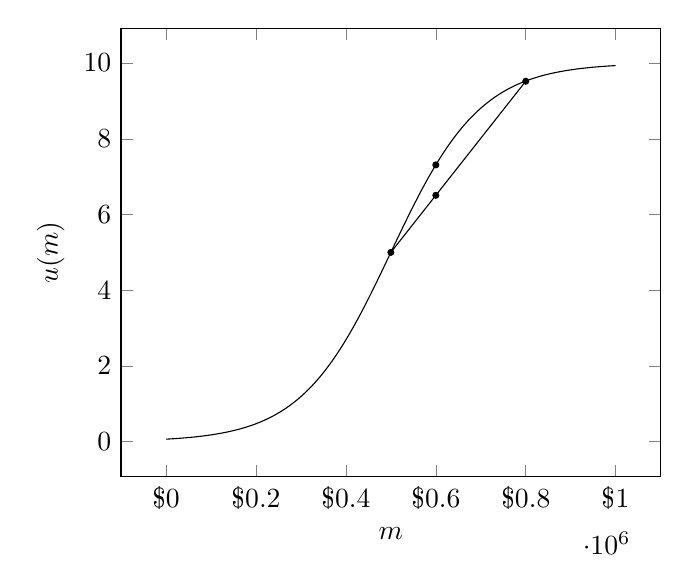
\begin{tikzpicture}
\begin{axis}[
    xlabel={$m$},
    ylabel={$u(m)$},
    xticklabel={\$$\pgfmathprintnumber{\tick}$},
    %title={A graphic interpretation of the gamble}
  ]
  \addplot[color=black,mark=none]
  coordinates {
(0,0.0669)(1000,0.0676)(2000,0.0683)(3000,0.069)(4000,0.0696)
(5000,0.0703)(6000,0.071)(7000,0.0717)(8000,0.0725)(9000,0.0732)
(10000,0.0739)(11000,0.0747)(12000,0.0754)(13000,0.0761)(14000,0.0769)
(15000,0.0777)(16000,0.0785)(17000,0.0792)(18000,0.08)(19000,0.0808)
(20000,0.0816)(21000,0.0824)(22000,0.0833)(23000,0.0841)(24000,0.0849)
(25000,0.0858)(26000,0.0866)(27000,0.0875)(28000,0.0884)(29000,0.0892)
(30000,0.0901)(31000,0.091)(32000,0.0919)(33000,0.0929)(34000,0.0938)
(35000,0.0947)(36000,0.0957)(37000,0.0966)(38000,0.0976)(39000,0.0985)
(40000,0.0995)(41000,0.1005)(42000,0.1015)(43000,0.1025)(44000,0.1035)
(45000,0.1046)(46000,0.1056)(47000,0.1067)(48000,0.1077)(49000,0.1088)
(50000,0.1099)(51000,0.111)(52000,0.1121)(53000,0.1132)(54000,0.1143)
(55000,0.1154)(56000,0.1166)(57000,0.1177)(58000,0.1189)(59000,0.1201)
(60000,0.1213)(61000,0.1225)(62000,0.1237)(63000,0.1249)(64000,0.1262)
(65000,0.1274)(66000,0.1287)(67000,0.13)(68000,0.1313)(69000,0.1326)
(70000,0.1339)(71000,0.1352)(72000,0.1365)(73000,0.1379)(74000,0.1393)
(75000,0.1406)(76000,0.142)(77000,0.1434)(78000,0.1449)(79000,0.1463)
(80000,0.1477)(81000,0.1492)(82000,0.1507)(83000,0.1522)(84000,0.1537)
(85000,0.1552)(86000,0.1567)(87000,0.1583)(88000,0.1598)(89000,0.1614)
(90000,0.163)(91000,0.1646)(92000,0.1663)(93000,0.1679)(94000,0.1696)
(95000,0.1712)(96000,0.1729)(97000,0.1746)(98000,0.1764)(99000,0.1781)
(1e+05,0.1799)(101000,0.1816)(102000,0.1834)(103000,0.1852)(104000,0.1871)
(105000,0.1889)(106000,0.1908)(107000,0.1927)(108000,0.1946)(109000,0.1965)
(110000,0.1984)(111000,0.2004)(112000,0.2023)(113000,0.2043)(114000,0.2063)
(115000,0.2084)(116000,0.2104)(117000,0.2125)(118000,0.2146)(119000,0.2167)
(120000,0.2188)(121000,0.221)(122000,0.2231)(123000,0.2253)(124000,0.2275)
(125000,0.2298)(126000,0.232)(127000,0.2343)(128000,0.2366)(129000,0.2389)
(130000,0.2413)(131000,0.2436)(132000,0.246)(133000,0.2484)(134000,0.2509)
(135000,0.2533)(136000,0.2558)(137000,0.2583)(138000,0.2608)(139000,0.2634)
(140000,0.266)(141000,0.2686)(142000,0.2712)(143000,0.2738)(144000,0.2765)
(145000,0.2792)(146000,0.282)(147000,0.2847)(148000,0.2875)(149000,0.2903)
(150000,0.2931)(151000,0.296)(152000,0.2989)(153000,0.3018)(154000,0.3047)
(155000,0.3077)(156000,0.3107)(157000,0.3137)(158000,0.3168)(159000,0.3198)
(160000,0.323)(161000,0.3261)(162000,0.3293)(163000,0.3325)(164000,0.3357)
(165000,0.339)(166000,0.3422)(167000,0.3456)(168000,0.3489)(169000,0.3523)
(170000,0.3557)(171000,0.3592)(172000,0.3626)(173000,0.3661)(174000,0.3697)
(175000,0.3733)(176000,0.3769)(177000,0.3805)(178000,0.3842)(179000,0.3879)
(180000,0.3917)(181000,0.3954)(182000,0.3993)(183000,0.4031)(184000,0.407)
(185000,0.4109)(186000,0.4149)(187000,0.4189)(188000,0.4229)(189000,0.427)
(190000,0.4311)(191000,0.4352)(192000,0.4394)(193000,0.4436)(194000,0.4479)
(195000,0.4522)(196000,0.4565)(197000,0.4609)(198000,0.4653)(199000,0.4698)
(2e+05,0.4743)(201000,0.4788)(202000,0.4834)(203000,0.488)(204000,0.4927)
(205000,0.4974)(206000,0.5021)(207000,0.5069)(208000,0.5117)(209000,0.5166)
(210000,0.5215)(211000,0.5265)(212000,0.5315)(213000,0.5366)(214000,0.5417)
(215000,0.5468)(216000,0.552)(217000,0.5572)(218000,0.5625)(219000,0.5679)
(220000,0.5732)(221000,0.5787)(222000,0.5841)(223000,0.5897)(224000,0.5952)
(225000,0.6009)(226000,0.6065)(227000,0.6123)(228000,0.618)(229000,0.6239)
(230000,0.6297)(231000,0.6357)(232000,0.6416)(233000,0.6477)(234000,0.6538)
(235000,0.6599)(236000,0.6661)(237000,0.6723)(238000,0.6786)(239000,0.685)
(240000,0.6914)(241000,0.6978)(242000,0.7044)(243000,0.7109)(244000,0.7176)
(245000,0.7243)(246000,0.731)(247000,0.7378)(248000,0.7447)(249000,0.7516)
(250000,0.7586)(251000,0.7656)(252000,0.7727)(253000,0.7799)(254000,0.7871)
(255000,0.7944)(256000,0.8017)(257000,0.8091)(258000,0.8166)(259000,0.8241)
(260000,0.8317)(261000,0.8394)(262000,0.8471)(263000,0.8549)(264000,0.8627)
(265000,0.8707)(266000,0.8786)(267000,0.8867)(268000,0.8948)(269000,0.903)
(270000,0.9112)(271000,0.9195)(272000,0.9279)(273000,0.9364)(274000,0.9449)
(275000,0.9535)(276000,0.9622)(277000,0.9709)(278000,0.9797)(279000,0.9886)
(280000,0.9975)(281000,1.0065)(282000,1.0156)(283000,1.0248)(284000,1.034)
(285000,1.0433)(286000,1.0527)(287000,1.0621)(288000,1.0717)(289000,1.0813)
(290000,1.091)(291000,1.1007)(292000,1.1106)(293000,1.1205)(294000,1.1305)
(295000,1.1405)(296000,1.1507)(297000,1.1609)(298000,1.1712)(299000,1.1816)
(3e+05,1.192)(301000,1.2026)(302000,1.2132)(303000,1.2239)(304000,1.2347)
(305000,1.2455)(306000,1.2565)(307000,1.2675)(308000,1.2786)(309000,1.2898)
(310000,1.3011)(311000,1.3124)(312000,1.3239)(313000,1.3354)(314000,1.347)
(315000,1.3587)(316000,1.3705)(317000,1.3824)(318000,1.3943)(319000,1.4064)
(320000,1.4185)(321000,1.4307)(322000,1.443)(323000,1.4554)(324000,1.4679)
(325000,1.4805)(326000,1.4931)(327000,1.5059)(328000,1.5187)(329000,1.5316)
(330000,1.5447)(331000,1.5578)(332000,1.571)(333000,1.5842)(334000,1.5976)
(335000,1.6111)(336000,1.6247)(337000,1.6383)(338000,1.652)(339000,1.6659)
(340000,1.6798)(341000,1.6938)(342000,1.708)(343000,1.7222)(344000,1.7365)
(345000,1.7509)(346000,1.7654)(347000,1.7799)(348000,1.7946)(349000,1.8094)
(350000,1.8243)(351000,1.8392)(352000,1.8543)(353000,1.8694)(354000,1.8847)
(355000,1.9)(356000,1.9155)(357000,1.931)(358000,1.9466)(359000,1.9623)
(360000,1.9782)(361000,1.9941)(362000,2.0101)(363000,2.0262)(364000,2.0424)
(365000,2.0587)(366000,2.0751)(367000,2.0916)(368000,2.1082)(369000,2.1249)
(370000,2.1417)(371000,2.1585)(372000,2.1755)(373000,2.1926)(374000,2.2097)
(375000,2.227)(376000,2.2444)(377000,2.2618)(378000,2.2794)(379000,2.297)
(380000,2.3148)(381000,2.3326)(382000,2.3505)(383000,2.3685)(384000,2.3867)
(385000,2.4049)(386000,2.4232)(387000,2.4416)(388000,2.4601)(389000,2.4787)
(390000,2.4974)(391000,2.5162)(392000,2.5351)(393000,2.554)(394000,2.5731)
(395000,2.5923)(396000,2.6115)(397000,2.6308)(398000,2.6503)(399000,2.6698)
(4e+05,2.6894)(401000,2.7091)(402000,2.7289)(403000,2.7488)(404000,2.7688)
(405000,2.7888)(406000,2.809)(407000,2.8292)(408000,2.8496)(409000,2.87)
(410000,2.8905)(411000,2.9111)(412000,2.9318)(413000,2.9525)(414000,2.9734)
(415000,2.9943)(416000,3.0153)(417000,3.0365)(418000,3.0576)(419000,3.0789)
(420000,3.1003)(421000,3.1217)(422000,3.1432)(423000,3.1648)(424000,3.1865)
(425000,3.2082)(426000,3.23)(427000,3.2519)(428000,3.2739)(429000,3.296)
(430000,3.3181)(431000,3.3403)(432000,3.3626)(433000,3.385)(434000,3.4074)
(435000,3.4299)(436000,3.4525)(437000,3.4751)(438000,3.4978)(439000,3.5206)
(440000,3.5434)(441000,3.5663)(442000,3.5893)(443000,3.6124)(444000,3.6355)
(445000,3.6586)(446000,3.6819)(447000,3.7052)(448000,3.7285)(449000,3.7519)
(450000,3.7754)(451000,3.7989)(452000,3.8225)(453000,3.8462)(454000,3.8699)
(455000,3.8936)(456000,3.9174)(457000,3.9413)(458000,3.9652)(459000,3.9891)
(460000,4.0131)(461000,4.0372)(462000,4.0613)(463000,4.0854)(464000,4.1096)
(465000,4.1338)(466000,4.1581)(467000,4.1824)(468000,4.2068)(469000,4.2311)
(470000,4.2556)(471000,4.28)(472000,4.3045)(473000,4.3291)(474000,4.3536)
(475000,4.3782)(476000,4.4029)(477000,4.4275)(478000,4.4522)(479000,4.4769)
(480000,4.5017)(481000,4.5264)(482000,4.5512)(483000,4.576)(484000,4.6009)
(485000,4.6257)(486000,4.6506)(487000,4.6755)(488000,4.7004)(489000,4.7253)
(490000,4.7502)(491000,4.7752)(492000,4.8001)(493000,4.8251)(494000,4.85)
(495000,4.875)(496000,4.9)(497000,4.925)(498000,4.95)(499000,4.975)
(5e+05,5)(501000,5.025)(502000,5.05)(503000,5.075)(504000,5.1)
(505000,5.125)(506000,5.15)(507000,5.1749)(508000,5.1999)(509000,5.2248)
(510000,5.2498)(511000,5.2747)(512000,5.2996)(513000,5.3245)(514000,5.3494)
(515000,5.3743)(516000,5.3991)(517000,5.424)(518000,5.4488)(519000,5.4736)
(520000,5.4983)(521000,5.5231)(522000,5.5478)(523000,5.5725)(524000,5.5971)
(525000,5.6218)(526000,5.6464)(527000,5.6709)(528000,5.6955)(529000,5.72)
(530000,5.7444)(531000,5.7689)(532000,5.7932)(533000,5.8176)(534000,5.8419)
(535000,5.8662)(536000,5.8904)(537000,5.9146)(538000,5.9387)(539000,5.9628)
(540000,5.9869)(541000,6.0109)(542000,6.0348)(543000,6.0587)(544000,6.0826)
(545000,6.1064)(546000,6.1301)(547000,6.1538)(548000,6.1775)(549000,6.2011)
(550000,6.2246)(551000,6.2481)(552000,6.2715)(553000,6.2948)(554000,6.3181)
(555000,6.3414)(556000,6.3645)(557000,6.3876)(558000,6.4107)(559000,6.4337)
(560000,6.4566)(561000,6.4794)(562000,6.5022)(563000,6.5249)(564000,6.5475)
(565000,6.5701)(566000,6.5926)(567000,6.615)(568000,6.6374)(569000,6.6597)
(570000,6.6819)(571000,6.704)(572000,6.7261)(573000,6.7481)(574000,6.77)
(575000,6.7918)(576000,6.8135)(577000,6.8352)(578000,6.8568)(579000,6.8783)
(580000,6.8997)(581000,6.9211)(582000,6.9424)(583000,6.9635)(584000,6.9847)
(585000,7.0057)(586000,7.0266)(587000,7.0475)(588000,7.0682)(589000,7.0889)
(590000,7.1095)(591000,7.13)(592000,7.1504)(593000,7.1708)(594000,7.191)
(595000,7.2112)(596000,7.2312)(597000,7.2512)(598000,7.2711)(599000,7.2909)
(6e+05,7.3106)(601000,7.3302)(602000,7.3497)(603000,7.3692)(604000,7.3885)
(605000,7.4077)(606000,7.4269)(607000,7.446)(608000,7.4649)(609000,7.4838)
(610000,7.5026)(611000,7.5213)(612000,7.5399)(613000,7.5584)(614000,7.5768)
(615000,7.5951)(616000,7.6133)(617000,7.6315)(618000,7.6495)(619000,7.6674)
(620000,7.6852)(621000,7.703)(622000,7.7206)(623000,7.7382)(624000,7.7556)
(625000,7.773)(626000,7.7903)(627000,7.8074)(628000,7.8245)(629000,7.8415)
(630000,7.8583)(631000,7.8751)(632000,7.8918)(633000,7.9084)(634000,7.9249)
(635000,7.9413)(636000,7.9576)(637000,7.9738)(638000,7.9899)(639000,8.0059)
(640000,8.0218)(641000,8.0377)(642000,8.0534)(643000,8.069)(644000,8.0845)
(645000,8.1)(646000,8.1153)(647000,8.1306)(648000,8.1457)(649000,8.1608)
(650000,8.1757)(651000,8.1906)(652000,8.2054)(653000,8.2201)(654000,8.2346)
(655000,8.2491)(656000,8.2635)(657000,8.2778)(658000,8.292)(659000,8.3062)
(660000,8.3202)(661000,8.3341)(662000,8.348)(663000,8.3617)(664000,8.3753)
(665000,8.3889)(666000,8.4024)(667000,8.4158)(668000,8.429)(669000,8.4422)
(670000,8.4553)(671000,8.4684)(672000,8.4813)(673000,8.4941)(674000,8.5069)
(675000,8.5195)(676000,8.5321)(677000,8.5446)(678000,8.557)(679000,8.5693)
(680000,8.5815)(681000,8.5936)(682000,8.6057)(683000,8.6176)(684000,8.6295)
(685000,8.6413)(686000,8.653)(687000,8.6646)(688000,8.6761)(689000,8.6876)
(690000,8.6989)(691000,8.7102)(692000,8.7214)(693000,8.7325)(694000,8.7435)
(695000,8.7545)(696000,8.7653)(697000,8.7761)(698000,8.7868)(699000,8.7974)
(7e+05,8.808)(701000,8.8184)(702000,8.8288)(703000,8.8391)(704000,8.8493)
(705000,8.8595)(706000,8.8695)(707000,8.8795)(708000,8.8894)(709000,8.8993)
(710000,8.909)(711000,8.9187)(712000,8.9283)(713000,8.9379)(714000,8.9473)
(715000,8.9567)(716000,8.966)(717000,8.9752)(718000,8.9844)(719000,8.9935)
(720000,9.0025)(721000,9.0114)(722000,9.0203)(723000,9.0291)(724000,9.0378)
(725000,9.0465)(726000,9.0551)(727000,9.0636)(728000,9.0721)(729000,9.0805)
(730000,9.0888)(731000,9.097)(732000,9.1052)(733000,9.1133)(734000,9.1214)
(735000,9.1293)(736000,9.1373)(737000,9.1451)(738000,9.1529)(739000,9.1606)
(740000,9.1683)(741000,9.1759)(742000,9.1834)(743000,9.1909)(744000,9.1983)
(745000,9.2056)(746000,9.2129)(747000,9.2201)(748000,9.2273)(749000,9.2344)
(750000,9.2414)(751000,9.2484)(752000,9.2553)(753000,9.2622)(754000,9.269)
(755000,9.2757)(756000,9.2824)(757000,9.2891)(758000,9.2956)(759000,9.3022)
(760000,9.3086)(761000,9.315)(762000,9.3214)(763000,9.3277)(764000,9.3339)
(765000,9.3401)(766000,9.3462)(767000,9.3523)(768000,9.3584)(769000,9.3643)
(770000,9.3703)(771000,9.3761)(772000,9.382)(773000,9.3877)(774000,9.3935)
(775000,9.3991)(776000,9.4048)(777000,9.4103)(778000,9.4159)(779000,9.4213)
(780000,9.4268)(781000,9.4321)(782000,9.4375)(783000,9.4428)(784000,9.448)
(785000,9.4532)(786000,9.4583)(787000,9.4634)(788000,9.4685)(789000,9.4735)
(790000,9.4785)(791000,9.4834)(792000,9.4883)(793000,9.4931)(794000,9.4979)
(795000,9.5026)(796000,9.5073)(797000,9.512)(798000,9.5166)(799000,9.5212)
(8e+05,9.5257)(801000,9.5302)(802000,9.5347)(803000,9.5391)(804000,9.5435)
(805000,9.5478)(806000,9.5521)(807000,9.5564)(808000,9.5606)(809000,9.5648)
(810000,9.5689)(811000,9.573)(812000,9.5771)(813000,9.5811)(814000,9.5851)
(815000,9.5891)(816000,9.593)(817000,9.5969)(818000,9.6007)(819000,9.6046)
(820000,9.6083)(821000,9.6121)(822000,9.6158)(823000,9.6195)(824000,9.6231)
(825000,9.6267)(826000,9.6303)(827000,9.6339)(828000,9.6374)(829000,9.6408)
(830000,9.6443)(831000,9.6477)(832000,9.6511)(833000,9.6544)(834000,9.6578)
(835000,9.661)(836000,9.6643)(837000,9.6675)(838000,9.6707)(839000,9.6739)
(840000,9.677)(841000,9.6802)(842000,9.6832)(843000,9.6863)(844000,9.6893)
(845000,9.6923)(846000,9.6953)(847000,9.6982)(848000,9.7011)(849000,9.704)
(850000,9.7069)(851000,9.7097)(852000,9.7125)(853000,9.7153)(854000,9.718)
(855000,9.7208)(856000,9.7235)(857000,9.7262)(858000,9.7288)(859000,9.7314)
(860000,9.734)(861000,9.7366)(862000,9.7392)(863000,9.7417)(864000,9.7442)
(865000,9.7467)(866000,9.7491)(867000,9.7516)(868000,9.754)(869000,9.7564)
(870000,9.7587)(871000,9.7611)(872000,9.7634)(873000,9.7657)(874000,9.768)
(875000,9.7702)(876000,9.7725)(877000,9.7747)(878000,9.7769)(879000,9.779)
(880000,9.7812)(881000,9.7833)(882000,9.7854)(883000,9.7875)(884000,9.7896)
(885000,9.7916)(886000,9.7937)(887000,9.7957)(888000,9.7977)(889000,9.7996)
(890000,9.8016)(891000,9.8035)(892000,9.8054)(893000,9.8073)(894000,9.8092)
(895000,9.8111)(896000,9.8129)(897000,9.8148)(898000,9.8166)(899000,9.8184)
(9e+05,9.8201)(901000,9.8219)(902000,9.8236)(903000,9.8254)(904000,9.8271)
(905000,9.8288)(906000,9.8304)(907000,9.8321)(908000,9.8337)(909000,9.8354)
(910000,9.837)(911000,9.8386)(912000,9.8402)(913000,9.8417)(914000,9.8433)
(915000,9.8448)(916000,9.8463)(917000,9.8478)(918000,9.8493)(919000,9.8508)
(920000,9.8523)(921000,9.8537)(922000,9.8551)(923000,9.8566)(924000,9.858)
(925000,9.8594)(926000,9.8607)(927000,9.8621)(928000,9.8635)(929000,9.8648)
(930000,9.8661)(931000,9.8674)(932000,9.8687)(933000,9.87)(934000,9.8713)
(935000,9.8726)(936000,9.8738)(937000,9.8751)(938000,9.8763)(939000,9.8775)
(940000,9.8787)(941000,9.8799)(942000,9.8811)(943000,9.8823)(944000,9.8834)
(945000,9.8846)(946000,9.8857)(947000,9.8868)(948000,9.8879)(949000,9.889)
(950000,9.8901)(951000,9.8912)(952000,9.8923)(953000,9.8933)(954000,9.8944)
(955000,9.8954)(956000,9.8965)(957000,9.8975)(958000,9.8985)(959000,9.8995)
(960000,9.9005)(961000,9.9015)(962000,9.9024)(963000,9.9034)(964000,9.9043)
(965000,9.9053)(966000,9.9062)(967000,9.9071)(968000,9.9081)(969000,9.909)
(970000,9.9099)(971000,9.9108)(972000,9.9116)(973000,9.9125)(974000,9.9134)
(975000,9.9142)(976000,9.9151)(977000,9.9159)(978000,9.9167)(979000,9.9176)
(980000,9.9184)(981000,9.9192)(982000,9.92)(983000,9.9208)(984000,9.9215)
(985000,9.9223)(986000,9.9231)(987000,9.9239)(988000,9.9246)(989000,9.9253)
(990000,9.9261)(991000,9.9268)(992000,9.9275)(993000,9.9283)(994000,9.929)
(995000,9.9297)(996000,9.9304)(997000,9.931)(998000,9.9317)(999000,9.9324)
(1e+06,9.9331)
  };
  \node (a) at (500000,5) [place] {};
  \node (b) at (800000,9.52) [place] {};
  \node at (600000,6.506667) [place] {};
  \node (c) at (600000,7.31) [place] {};
  \draw [-] (a) -- (b);
\end{axis}
\end{tikzpicture}
\caption{A graphic interpretation of the gamble.}
\label{fig:gamble}
\end{figure}

We can represent the situation graphically by drawing a line segment
from the utility when losing
$u(\$\num{500000})$ to the utility when winning
$u(\$\num{800000})$, and noting the point at one-third of the distance
from $u(\$\num{500000})$ to
$u(\$\num{800000})$ (see figure~\vref{fig:gamble}).  The corresponding
monetary value is the expected value of the gamble,
i.e. \$\num{600000}, and the corresponding utility is the expected
utility of the gamble, 6.51. With \$\num{600000} in retirement funds,
Alice's behavior changes.  We say that her utility function is
risk-averse (or concave) in the range from \$\num{500000} to
\$\num{1000000} and that it is risk-seeking (or convex) in the range
from \$0 to \$\num{500000}.

Notice that if Alice had only \$\num{100000} in retirement savings,
then her utility would be 0.180 and her utility for the gamble would
be
\[
\frac{1}{3}u(\$\num{300000}) + \frac{2}{3}u(\$\num{0}) = 0.442.
\]
With \$\num{100000} in retirement funds, Alice cannot fund the
lifestyle that she desires and she would be willing to gamble even
when it could be slightly unfavorable for her to do
so\footnote{Homeowner's insurance is another example where people
  engage in gambles (or lotteries) that are unfavorable in
  expectation.}.  At this point, one might object that most people do
not gamble with retirement savings. However, we have not described the
utility function for most people; we have described the utility
function for Alice. Recall that a utility function is used to
(numerically) represent a decision-maker's preferences over outcomes.
If Alice was risk-averse with all of her retirement savings, then the
shape of her utility function would be risk-averse over the entire
domain.

\begin{comment}
\emph{Exercise 2.} Suppose Mr. Campbell has \$3. He is offered a fair bet
in which he wins \$2 with probability 1/3 or he loses \$1 with
probability 2/3. Should accept the bet? Suppose he is offered a
compound bet where win or lose he must repeat the above bet a second
time.  Should he accept the compound bet? What condition of the
Expected Utility Theorem should Mr. Campbell apply to his decision 
on whether to accept the compound bet?

\emph{Exercise 3.} Mrs. Campbell escorts her husband to sky-diving
school. For \$50 she can get \$5000 worth of insurance. Mr.  Campbell
laughs and says ``no''. He fully expects that nothing will go
wrong. Besides, he took both IE~3521 and IE~5545 and so he says that
the insurance company makes a profit by not giving people their
money's worth in insurance. Now, Mrs. Campbell makes her own
decisions. Should she purchase the insurance? Give an argument for or
against the insurance, and make use of utilities that you think are
reasonable.
\end{comment}

\section{Exercises}
\begin{enumerate}

% written by Emily	
\item \emph{Structuring a decision problem.} 
An online retail company is looking to purchase some robots to
perform tasks in their warehouse. There are two types of 
helpful robots available. Robot A can collect
items in the warehouse. Robot B seals boxes shut. Robot A costs \$\num{6000}
and Robot B costs \$\num{3000}.
The business has \$\num{15000} available to spend and they value money. 
The money-equivalent
value (payoff) they get from acquiring their first Robot A is 
\$\num{14000} and
that of each additional Robot A is half the previous one (the second
Robot A gives them a value of \$\num{7000}, the third \$\num{3500} and so on).
Similarly, the payoff they get from acquiring their first Robot B is
\$\num{5000} and that of each additional Robot B is half the previous one
(\$\num{2500}, \$\num{1250}, \ldots). The robots do separate jobs, so 
the value from each Robot A acquired is not
affected by how many of Robot B are acquired, and vice versa.

\begin{enumerate}
\item Draw the decision tree that is associated with this problem. 
\item The business makes decisions based on maximizing their 
payoff. Should they spend all of their available money on 
these robots?
\end{enumerate}

Compute the payoff for each leaf (or end--node) of the
decision tree. For example, if you purchase one Robot A and one
Robot B, you will spend \$\num{9000} and the payoff is
  \[ \num{15000}-\num{6000}-\num{3000} + \num{14000}+\num{5000} = \$\num{25000} \]
  Note that I included the initial amount of available
  cash in the calculation because the problem states 
  ``\ldots and you value money.''

\begin{solution}
\bs
In the tree below, ``A'' indicates a choice for number of 
Robot A to purchase, and ``B'' indicates a choice for number 
of Robot B to purchase.

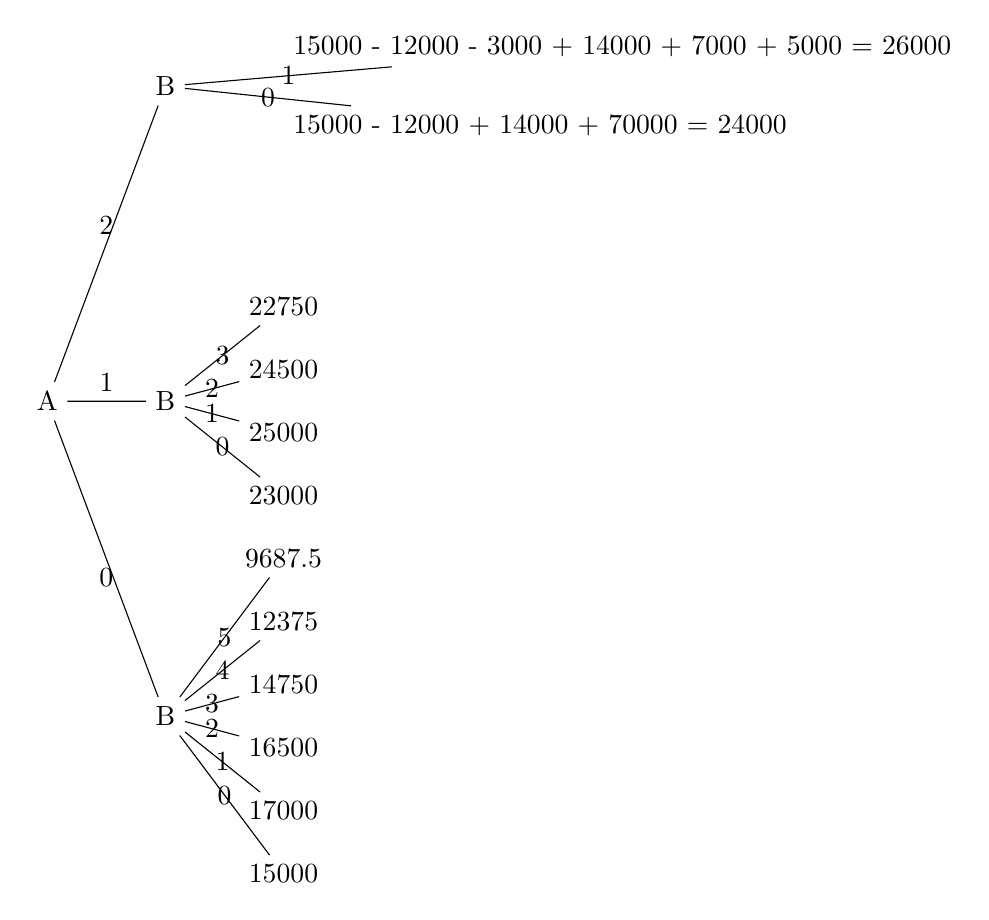
\begin{tikzpicture}
  \tikzstyle{level 1}=[sibling distance=40mm]
  \tikzstyle{level 2}=[sibling distance=8mm]
  \node {A} [grow=right]
  child{node {B} 
    child {node {\num{15000}}
    edge from parent node {0}}
    child {node {\num{17000}}
    edge from parent node {1}}
    child {node {\num{16500}}
    edge from parent node {2}}
    child {node {\num{14750}}
    edge from parent node {3}}
    child {node {\num{12375}}
    edge from parent node {4}}
    child {node {\num{9687.5}}
    edge from parent node {5}}
    edge from parent node[below] {0} }
  child {node {B}
    child {node {\num{23000}}
    edge from parent node {0}}
    child {node {\num{25000}}
    edge from parent node {1}}
    child {node {\num{24500}}
    edge from parent node {2}}
    child {node {\num{22750}}
    edge from parent node {3}}
    edge from parent node[above] {1} }
  child {node {B}
    child[sibling distance=10mm] {node[anchor=west] {\num{15000} -
    \num{12000} + \num{14000} + \num{70000} = \num{24000}}
    edge from parent node {0}}
    child[sibling distance=10mm] {node[anchor=west] {\num{15000} - 
    \num{12000} - \num{3000} + \num{14000} + \num{7000} + \num{5000} 
    = \num{26000}}
    edge from parent node {1}}
    edge from parent node[above] {2} }
  ;
\end{tikzpicture}

The company wants to make the most rational decision, so they
choose the action that maximizes the payoff. 
The company should spend the entire \$\num{15000} on robots for 
their warehouse. They should purchase two of Robot A and one of 
Robot B for a money-equivalent value of \$\num{26000}.

\end{solution}

% This exercise is OK
\item \emph{Rules for decision--making under ignorance.}
  You have the opportunity to go on a
  blind date, but you are hesitant.  You are lonely and would like to
  find the love of your life; however, you dislike awkward
  situations. Furthermore, you find it difficult to estimate the
  probability that this particular blind date will turn out to be the
  love of your life, but you know this probability is
  non-negligible. To be a little more precise, you have the following
  values: finding the love of your life is worth 1000, being in an
  awkward date situation (i.e. being on a date and knowing that you
  will not see the person again) is worth -10, and staying home
  watching Netflix is worth zero.

\begin{enumerate}
\item Formulate a decision problem for deciding whether to go on the
blind date or to stay home.
\item Use the maximin rule to solve the problem.
\item Use the minimax regret rule to solve the problem.
\end{enumerate}

\begin{solution}
\bs The decision problem can be represented with the following table.
\\[.1in]
\begin{tabular}{ccc}
 \multicolumn{3}{c}{decision matrix} \\
 & find love & lots of awkward moments \\ \cline{2-3}
go on date & 1000 & -10 \\
decline date & 0 & 0 
\end{tabular}
\\[.1in] 
The maximin rule tells you to decline the date because it has
the best of all the worst possible outcomes. To use minimax regret, we
form the regret matrix.  \\[.1in]
\begin{tabular}{ccc}
 \multicolumn{3}{c}{regret matrix} \\
 & find love & lots of awkward moments \\ \cline{2-3}
go on date & 0 & -10 \\
decline date & -1000 & 0
\end{tabular}
\\[.1in] Minimax regret tells you to go on the date because the
possibility of not finding love has the most regret.
\end{solution}


\subsubsection*{Games Against Nature}

% written by Emily
\item \emph{Gardening against nature.} A family is considering growing
  their own garden to save money on fresh vegetables. They have space
  in their yard for the garden but would need to purchase seeds and
  gardening supplies. The family is excited to grow a garden, but they
  know there are a lot of hungry rabbits in their neighborhood that
  might eat their plants before the family can harvest any vegetables
  from them. Money saved by the garden is shown in the following
  table.

\begin{tabular}{rcc}
& \multicolumn{2}{c}{State of Nature} \\
& $s_1$ & $s_2$ \\
& rabbits leave garden alone & rabbits eat garden \\ \cline{2-3}
plant garden & \$400 & -\$100\\
buy vegetables from store & 0 & 0
\end{tabular}

\begin{enumerate}
    \item If the probability that the rabbits leave the garden alone is 0.3, what decision is recommended for the family? What are the expected savings?
    
    \item The family has the option to purchase fast-growing plant seeds (the fast-growing seeds are the same price as regular seeds but they must buy the fast-growing seeds now if they want them because they are in high demand).  With these fast-growing seeds, the family can wait three more weeks to plant their garden. During that time, some scientists will finish their study on the appetites of the local rabbits, and the family will have a better idea about the probability that their garden is eaten by rabbits. They can return the seeds later for a partial refund if they do not use them.
    Let $L$ represent the event the rabbits have large appetites and let $S$ represent
    the event that rabbits have small appetites. Then
    \[
    \begin{matrix}
    P(L)=0.60, & P(s_1 \mid L)=0.15, & P(s_2 \mid L)=0.85,\\
    P(S)=0.40, & P(s_1 \mid S)=0.79, & P(s_2 \mid S)=0.21.
    \end{matrix}
    \]
    What is the optimal decision strategy if the family purchases the fast-growing seeds so they can wait and learn more about the rabbit appetites before making a decision?
    
    \item If \$40\ of the fast-growing seed purchase is non-refundable, should the family purchase the fast-growing seeds? Why or why not? What is the maximum non-refundable amount the family should pay to get the fast-growing seeds?
\end{enumerate}

\begin{solution}
\bs For part a), the expected savings when planting the garden are
\[ 400 \times 0.3  - 100 \times 0.7 = \$50. \]
The savings from not planting the garden are \$0, so based on expected value,
the best decision is to plant the garden.

For part b), if the rabbits have large appetites ($L$), then planting 
the garden would result in -\$25 of expected savings.
If the rabbits have small appetites ($S$), then planting the garden will result in \$295 
of expected savings. 

If L, \[ \$100 \times 0.15 - \$100 \times 0.85 = -\$25 \]
If S, \[ \$400 \times 0.79 - \$100 \times 0.21 = \$295 \]

Not planting will always result in \$0 of savings. 
The optimal decision strategy is to plant the garden if $S$ and buy vegetables 
from the store if $L$.

For part c), we use the optimal decision for each possible event $L$ and $S$. 
The expected savings from purchasing the fast-growing seeds
(but before actually purchasing the seeds) are
\[ \$0 \times 0.60 + \$295 \times 0.40 = \$118 \]
The maximum non-refundable amount that the family should be willing 
to pay for the fast-growing seeds is
\[ \$118 - \$50 = \$68 \]
\end{solution}

% this problem is OK
\item \emph{Using Baye's formula to update a prior belief.}
Curling is a sport in which players slide a stone over ice toward a
target. The association governing the sport has implemented drug
testing. It is believed that 15\% of all curlers use banned drugs to
enhance performance. If a player uses banned drugs, the association
may take away any prizes that the player has won; however, it
undesirable to falsely accuse someone of using banned substances.  The
utilities for each decision and state of nature are

\begin{center}
\begin{tabular}{rrrr}
& drug use & no drug use \\ \cline{2-3}
take away prizes & -100 & -1000 \\
do not & -600 & 0 
\end{tabular}
\end{center}

Notice that there is a small dis-utility for taking prizes away from a drug user
due to bad publicity for the sport. The test to detect drug use is
less than 100\% reliable. In particular, if $D$ indicates that a 
player uses banned drugs, and $+$/$-$ indicate a positive/negative
test result, then the true positive rate and the true negative rate
are
\[
P(+ \mid D) = .97 \quad \text{and} \quad P(- \mid \overline{D}) = .97,
\]
respectively, Given the utilities and the accuracy of the test, what is the best
decision if a player has a positive test result? (The association
wants to maximize expected utility.)

\begin{solution}
\bs First we update the probability of drug use via Baye's formula.
\begin{align*}
P(D \mid +) &= \frac{P(D \cap +)}{P(+)} \\
&= \frac{P(+ \mid D)P(D)}{P(+ \mid D)P(D) + P(+ \mid \overline{D})P(\overline{D})} \\
&= \frac{.97 \times .15}{.97 \times .15 + .03 \times .85} \\
&= .851
\end{align*}
and then we can compute $P(\overline{D} \mid +) = 1 - P(D \mid +) = .149$.
Using these posterior probabilities, the expected utilities are
\begin{align*}
E(\text{take away}) &= (-100)(.851) + (-1000)(.149) = -234 \\
E(\text{do not}) &= (-600)(.851) = -511
\end{align*}
The best decision is to take away prizes when a player tests positive.
\end{solution}

% Emily - expected value and sensitivity analysis
\item \emph {Decisions under risk and sensitivity analysis.}  The
  owners of a popular outdoor furniture company predict that their
  sales will double this coming year. The company is already producing
  the maximum amount of furniture possible in their current
  facility. They are considering expanding their manufacturing
  facility to accommodate the predicted increase in demand. If
  undertaken, the expansion will cost \$\num{500000}. If the demand
  doubles as predicted, revenue will increase by \$\num{800000}.  If
  the predicted increase in demand proves to be too optimistic,
  revenue will increase by only \$\num{250000}.  If the expansion is
  not undertaken, the company will lose \$\num{50000} due to
  out-of-stock orders from agitated customers.  The change in demand
  will be determined by next year's weather; more outdoor furniture is
  sold when the weather is nice.  There is a 0.55 chance of good
  weather, which will result in a doubling of demand. There is a 0.45
  chance of poor weather, which will result in only a slight increase
  in demand.

\begin{enumerate}
\item Should the manufacturing facility be expanded? The owners make
  decisions based on expected value.
\item How does the decision change with the probability of good/poor
  weather? To answer this question, you should perform a sensitivity
  analysis.
\end{enumerate}

\begin{solution}
\bs The decision table for this problem is
\begin{center}
\begin{tabular}{rrr}
      & $0.55$ & $0.45$ \\
      & good weather & poor weather \\ \hline
      expansion & \$\num{300000} & -\$\num{250000} \\
      no expansion & -\$\num{50000} & -\$\num{50000}
\end{tabular}
\end{center}

The expected payoff of each decision is
\begin{align*}
&E(\text{expansion}) = 0.55 \times \$\num{300000}
- 0.45 \times \$\num{250000} = \$\num{52500} \\
&E(\text{no expansion}) = -\$\num{50000}
\end{align*}
The company should expand the facility. As the probability of poor
weather increases, the expected value of the expansion
decreases.  Let $p$ represent the probability of poor weather.
\begin{align*}
E(\text{expansion}) &= \num{300000}(1-p) - \num{250000}p \\
&= \num{300000} - \num{550000}p
\end{align*}
The company should expand the facility as long as
\begin{align*}
E(\text{expansion}) &\geq E(\text{no expansion}) \\
\num{300000} - \num{550000}p &\geq -\num{50000} \\
-\num{5500000}p &\geq -\num{350000} \\
p &\leq \frac{7}{11} \approx .64
\end{align*}
Expanding the facility is the best decision unless the probability of
poor weather is greater than .64.
\end{solution}

\item \emph{The value of perfect information.}  You are taking a 
  date to a movie. You like horror movies but you are unsure whether
  your date likes them. You have two choices for the movie, ``The
  Burrowers'' which, despite its title, you've heard is a good movie,
  and ``A Star is Born'', which is rather safe as far as date movies
  go. Your decision problem with associated payoffs is

\begingroup
\setlength{\tabcolsep}{9pt}
\renewcommand*{\arraystretch}{2}
\begin{tabularx}{4in}{YYY}
& \multicolumn{2}{c}{Your date} \\
& likes horror movies & hates horror movies\\ \cline{2-3}
\gtcol{The Burrowers} & \gtcol{10} & \gtcol{1} \\ \cline{2-3}
\gtcol{A Star is Born} & \gtcol{4} & \gtcol{7} \\ \cline{2-3}
\end{tabularx}
\endgroup

\vspace{.2in}
\begin{enumerate}
\item Let $p$ represent the probability that your date likes horror movies. What is
  the optimal decision as a function of $p$?
\item At this point you have no information for your date's movie
  preference (even the trail of social media cannot help you) and so
  you assign $p=1/2$ as your subjective prior probability. Suppose
  that the date's best friend will tell you for sure whether your date
  likes horror movies, but this person is not so nice and wants to be
  paid. If the payoffs represent dollar amounts then how much are you
  willing to pay this person for perfect information? \label{ex:pi}
\end{enumerate}

\begin{solution}
  \bs Choose ``The Burrowers'' if
  \begin{align*}
    10p + (1-p) &> 4p + 7(1-p)\\
    9p + 1 &> -3p + 7\\
    12p &> 6\\
    p &> 1/2
  \end{align*}

  Regarding part \ref{ex:pi}, if you knew that your date liked horror
  movies you would choose ``The Burrowers'' for a pyoff of \$10 and if
  you knew the opposite then you would choose ``A Star is Born'' for a
  payoff of \$7. The expected payoff with perfect information, that
  is, before you actually receive the information, is
  \[ \frac{1}{2}(10) + \frac{1}{2}(7) = 8\frac{1}{2} \]
  Without the information your expected payoff is $\$5 \frac{1}{2}$ (for either
  choice). You would be willing to pay at most
  \[ \$8.50 - \$5.50 = \$3 \]
  for the perfect information.

\end{solution}

% written by Emily
\item \emph{Quality control and the value of perfect information.} 
  A worker in a factory producing potato chips notices that a small 
  bolt is missing off of a piece of equipment in the packaging 
  area and determines that it fell into a bag before it was
  sealed. Two pallets worth of chips have been produced since 
  the last routine check was performed determining that the 
  bolt was in place. The worker does not want to throw away all
  bags of chips that the bolt could possibly be in, so he decides
  to search for the bolt. He has to decide if he should start 
  searching bags on pallet one or pallet two. If the bolt fell into
  a bag on pallet one and he searches bags on pallet one, there is a 0.5 
  chance of finding it by the end of the day. If the bolt fell into 
  a bag on pallet two and he searches pallet two, there is a 0.8 chance
  that he finds the bolt. The worker's prior probability that the bolt
  is in a bag on pallet one is 0.7 (he thinks it was loose from some work done earlier in the day and fell off right away).

\begin{enumerate}
\item The worker only has time to search one pallet per day. 
  In which pallet, one or two, should he look for the bolt?  
  The worker wants to maximize his
  probability of finding the bolt. 
\item Suppose that at the end of the day when the worker goes home,
  he has not found the bolt yet. Which pallet should he 
  search on day 2?
  \emph{Hint}: First update the prior probabilities that the bolt is
  in pallet one/two.
\item Suppose that on the second day, just before the worker begins
  to
  search for the bolt, a security guard approaches and tells him
  that he has access to security camera footage that would reveal when 
  the bolt fell into a bag (revealing which pallet the bolt is in).
  How much should the worker be willing to pay for this perfect 
  information?  Note that the ``units'' for the payment are in 
  terms of probabilities.
\end{enumerate}

\begin{solution}
\bs
Let $A$ be the event that the bolt is in pallet one and let $B$ be the event
that the bolt is in pallet two. Also, let $F_A$ represent the event that the worker
finds the bolt in pallet one (and similarly define $F_B$). We are given the
following.
\begin{align*}
  P(F_A \mid A) = 0.5 &\qquad P(\overline{F}_A \mid A) = 0.5 \\
  P(F_B \mid B) = 0.8 &\qquad P(\overline{F}_B \mid B) = 0.2 \\
\end{align*}

The worker's decision problem is

\begingroup
\setlength{\tabcolsep}{9pt}
\renewcommand*{\arraystretch}{2}
\begin{tabularx}{3.25in}{YYYY}
& & \multicolumn{2}{c}{Nature} \\
& & $0.7$ & $0.3$ \\
& & $A$ & $B$  \\ \cline{3-4}
\multirow{2}{.9in}{Worker} & \gtcol{Look in A} & \gtcol{.5} & \gtcol{0} \\ \cline{3-4}
& \gtcol{Look in B} & \gtcol{0} & \gtcol{.8} \\ \cline{3-4}
\end{tabularx}
\endgroup
\vspace{.2in}

The best option is to look in pallet one. He will find the bolt on the first
day with probability $0.7 \times 0.5 = 0.35$.

On the second day, the worker's belief that the bolt is in pallet one is updated to
\begin{align*}
  P(A \mid \overline{F}_A) &= \frac{P(\overline{F}_A \mid A)P(A)}{P(\overline{F}_A \mid A)P(A) + P(\overline{F}_A \mid B)P(B)}\\
                           &= \frac{0.5 \times 0.7}{0.5 \times 0.7 + 1 \times 0.3} \\
                           &= 0.538
\end{align*}
which implies that $P(B \mid \overline{F}_A) = 1 - 0.538 = 0.462$. On day two,
the worker's decision problem is

\begingroup
\setlength{\tabcolsep}{9pt}
\renewcommand*{\arraystretch}{2}
\begin{tabularx}{3.25in}{YYYY}
& & \multicolumn{2}{c}{Nature} \\
& & $0.538$ & $0.462$ \\
& & $A$ & $B$  \\ \cline{3-4}
\multirow{2}{.9in}{Worker} & \gtcol{Look in A} & \gtcol{.5} & \gtcol{0} \\ \cline{3-4}
& \gtcol{Look in B} & \gtcol{0} & \gtcol{.8} \\ \cline{3-4}
\end{tabularx}
\endgroup
\vspace{.2in}

and his best option is to look in pallet two. The worker will find the bolt with probability
\[ 0.462 \times 0.8 = 0.37\]

With perfect information, but \emph{before} receiving the information, the worker's
expected value for the probability of finding the bolt is
\[ 0.5 \times 0.538 + 0.8 \times 0.462 = 0.639 \]
and in terms of probability ``units'', he should be willing to pay
\[ 0.639 - 0.37 = 0.269 \]
for the information.

\end{solution}


% this problem is OK.
\item \emph{Planting crops and the value of imperfect information.} A
  farmer can plant one of four crops. The yield in bushels per acre
  depends on the particular crop planted and the weather during the
  growing season. Regarding crop yields, the weather can be
  categorized as dry, moderate, or wet. The estimated crop yields,
  commodity prices, and weather forecast are provided in the table
  below.

\begin{center}
\begin{tabular}{lcccc}
& dry & moderate & wet & \$/bushel \\ \hline
crop 1 & 30 & 50 & 60 & \$3.00 \\
crop 2 & 25 & 30 & 40 & \$4.50 \\
crop 3 & 40 & 35 & 35 & \$3.00 \\
crop 4 & 60 & 60 & 60 & \$1.50 \\ \hline
forecast & .2 & .5 & .3 & 
\end{tabular}
\end{center}

\begin{enumerate}
\item If the farmer maximizes expected monetary value, which crop
should she plant and what is her expected revenue per acre?

\item Suppose that the farmer could pay an oracle to tell her
with certainty which category of weather would occur during
the growing season. How much should the farmer be willing to 
pay for this perfect information? Your answer should be in terms
of \$/acre. \label{b}

\item Now suppose a start-up company that specializes in predictive
  modeling announces a new machine learning algorithm for weather
  forecasting. The predictions from the model are good, but not
  perfect.  In particular, the company advertises the following
  accuracy for the weather forecasting model. \label{c}

\begin{center}
\begin{tabular}{clccc}
& & \multicolumn{3}{c}{actual} \\
& & dry & moderate & wet \\ \cline{2-5}
\parbox[t]{2mm}{\multirow{3}{*}{\rotatebox[origin=c]{90}{model}}} & dry & .9 & .1 & .05 \\
& moderate & .05 & .8 & .05 \\
& wet & .05 & .1 & .9 
\end{tabular}
\end{center}

For example, if the weather actually turns out to be dry, the model
would have predicted dry weather with probability .9, moderate weather
with probability .05, and wet weather with probability .05. How much
should the farmer be willing to pay (again in \$/acre) for this
less-than-perfect prediction of the weather? Settle in with a cup of
coffee: this part requires some work. Here is a strategy.
\begin{enumerate}[i)]
\item Develop a notation, e.g., $x$ indicates the weather during the growing season,
and $x'$ indicates the prediction, where $x$ is dry, moderate, or wet.

\item Use Baye's formula to compute the posterior probabilities for
  each weather category given the predictions, e.g. you want to know
  $P(d \mid d')$, $P(m \mid d')$, etc.

\item Determine the expected payoff for each case that the prediction is
dry, moderate, and wet.

\item The expected value of the prediction (i.e. the expected value of the
less-than-perfect information) is the difference between the expected payoff
with the information and without it.
\end{enumerate}

\end{enumerate}

\begin{solution}
\bs Considering the estimated commodity prices, the payoff table and expected
values in \$/acre for each crop are

\begin{center}
\begin{tabular}{lrrrr}
& dry & moderate & wet & $E(\text{payoff})$ \\ \hline
crop 1 & 90 & 150 & 180 & \$147 \\
crop 2 & 112.5 & 135 & 180 & \$144 \\
crop 3 & 120 & 105 & 105 & \$108 \\
crop 4 & 90 & 90 & 90 & \$90 
\end{tabular}
\end{center}

To maximize expected monetary value the farmer should plant crop 1 and
expect \$147/acre of revenue. For part~\ref{b}, if she knew for
certain that the weather would be dry, moderate, or wet, then she
would plant crop 3 with revenue \$120 per acre, crop 1 with revenue
\$150 per acre, and crop 1 (or 2) with revenue \$180 per acre,
respectively. Prior to learning the perfect information, the farmer's
expected payoff with the new information is
\[
.2 \times \$120 + .5 \times \$150 + .3 \times \$180 = \$153
\]
and so the value of the perfect information is worth no more than
\[
\$153 - \$147 = \$6~\text{per acre}
\]

Now for part~\ref{c}, the likelihoods are provided as follows
(using the notation given in the problem description).
\[
\begin{matrix}
P(d' \mid d)=.9 & P(m' \mid d)=.05 & P(w' \mid d)=.05 \\
P(d' \mid m)=.1 & P(m' \mid m)=.8 & P(w' \mid m)=.1 \\
P(d' \mid w)=.05 & P(m' \mid w)=.05 & P(w' \mid w)=.9 \\
\end{matrix}
\]

Using Baye's formula to compute the posterior probabilities, we get
\begin{align*}
P(d \mid d') &= \frac{P(d \cap d')}{P(d')} \\
&= \frac{P(d' \mid d)P(d)}{P(d' \mid d)P(d) + P(d' \mid m)P(m) + P(d' \mid w)P(w)} \\
&= \frac{(.9)(.2)}{(.9)(.2) + (.1)(.5) + (.05)(.3)} \\
&= .735
\end{align*}
and in a similar manner 
\[
\begin{matrix}
& P(m \mid d')=.204 & P(w \mid d')=.061 \\
P(d \mid m')=.024 & P(m \mid m')=.941 & P(w \mid m')=.035 \\
P(d \mid w')=.03 & P(m \mid w')=.152 & P(w \mid w')=.818 \\
\end{matrix}
\]
The expected monetary values given the predictions are

\begin{center}
\begin{tabular}{lrrr}
& $E(\text{dry})$ & $E(\text{moderate})$ & $E(\text{wet})$ \\ \hline
crop 1 & \$108 & 150 & 173 \\
crop 2 & 121 & 136 & 171 \\
crop 3 & 116 & 105 & 105 \\
crop 4 & 90 & 90 & 90
\end{tabular}
\end{center}

If the prediction is dry, the farmer would plant crop 2 for an
expected revenue of \$121 per acre. Similarly for predictions
of moderate and wet, she would plant crop 1 with expected revenue
\$150 per acre and crop 1 with expected revenue \$173 per acre,
respectively. Prior to obtaining the weather prediction,
the expected value of having the prediction is 
\begin{align*}
E(\text{payoff}) &= \$121 \times P(d') + \$150 \times P(m') + \$173 \times P(w') \\
&= \$121 \times .245 + \$150 \times .425 + \$173 \times .33 \\
&= \$150.50
\end{align*}
Note that the unconditional probabilities of the predictions are obtained
using the formula for total probability and they were computed during the
application of Baye's formula. The value of the less-than-perfect
informtaion is 
\[
\$150.50 - \$147 = \$3.50~\text{per acre}
\]
\end{solution}

% decisions over time
% this problem is OK.
\item \emph{The break-up.} You are considering
  breaking up with your boy(girl)friend; however, you know that
  he(she) may break up with you. Your utility is higher if you end
  the realtionship, but it's Friday and you have joint plans for the
  weekend. Here is the situation: on Friday (and possibly Saturday)
  you need to decide to either stay in the relationship, or end it.
  \begin{compactitem}[i)]
    \item \emph{On Friday:}
  If you decide to end the relationship your payoff is one
  (and your done.) If you stay in the relationship then a random
  chance event happens where your boy(girl)friend ends the relationship
  with probability 0.25 and stays with probability 0.75.
\item \emph{On Saturday:} If you end the relationship your
  payoff is 3 (and your done.) If you stay then a chance event happens
  where your boy(girl)friend ends the relationship with probability
  0.5 and stays with probability 0.5.
\end{compactitem}
If you stay in the relationship until Sunday, then you will definitely
end it and your payoff is 4. If, on Friday or Saturday, your boy(girl)friend
ends the relationship then your payoff is one.

Use backward induction to determine a policy for ending/staying that
will maximize your expected payoff.

\begin{solution}
  \bs The decision tree is shown below. Working backwards, the expected
  value of ``stay'' on Saturday is 2.5, so the best decision is ``exit'',
  for a payoff of 3. On Friday, the expected value of ``stay'' is 2.5,
  which is better than ``exit'' with a payoff of 1. So, the policy that
  maximizes expected payoff is to stay in the relationship on Friday and
  exit the relationship on Saturday.

\vspace{.2in}
\begin{center}
%\resizebox{.5\textwidth}{!}{%
  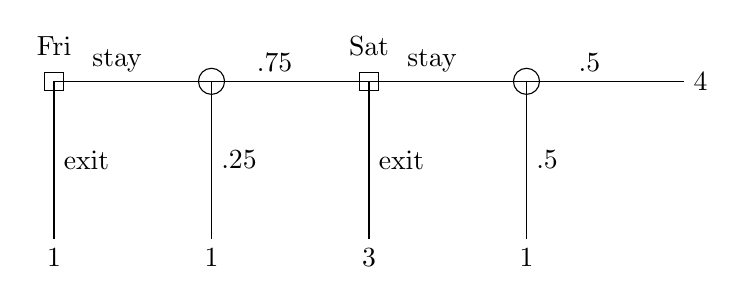
\begin{tikzpicture}
    \draw (0,0) -- (8,0)
    node[pos=.1,anchor=south] {stay}
    node[pos=.35,anchor=south] {.75}
    node[pos=0.6,anchor=south] {stay}
    node[pos=.85,anchor=south] {.5}
    node[right] {4};
    \draw (0,0) -- (0,-2) node[pos=0.5,anchor=west] {exit} node[below] {1};
    \draw (2,0) -- (2,-2) node[pos=.5,anchor=west] {.25} node[below] {1};
    \draw (4,0) -- (4,-2) node[pos=0.5,anchor=west] {exit} node[below] {3};
    \draw (6,0) -- (6,-2) node[pos=0.5,anchor=west] {.5} node[below] {1};
    \node[draw] at (0,0) {};
    \node[circle,draw] at (2,0) {};
    \node[draw] at (4,0) {};
    \node[circle,draw] at (6,0) {};
    \node[anchor=south] at (0,0.2) {Fri};
    \node[anchor=south] at (4,0.2) {Sat};
\end{tikzpicture}%}
\end{center}
\end{solution}

% written by Emily
\item \emph{An optimal strategy for a family visit.}  
Parker's family is 
coming to visit him for two days. He is going to plan an activity 
for each day, and he must decide if it will be an indoor
or outdoor activity. What he chooses the first day (indoor or
outdoor) can differ from what he chooses the second day. He wants
his family to enjoy whatever he chooses. There are many factors
that determine if Parker's family enjoys an activity such as
weather, how they are feeling, and their interest level.
If Parker picks an outdoor activity, the probability that
his family will enjoy the activity is $p_e$ and the probability
that they do not enjoy the activity is $1-p_e$.
If Parker picks an indoor activity, the probability that his family will 
enjoy the activity is $p_h$ and the probability that they will not 
is $1-p_h$. 
To measure the success of the visit, Parker has come up with the 
following scoring system: an outdoor activity that his family enjoys 
is worth 2 points, an indoor activity that his family enjoys is worth 
1 point, and any activity that his family does not enjoy is worth 
zero points.
Let $p_e=0.4$ and let $p_h=0.75$. 
Which type of activity should Parker select for the first day
of the visit, indoor or outdoor? What about the second day? 
In other words, what is the
plan that will maximize Parker's expected 
payoff for the 2-day visit?

\begin{solution}
  \bs The optimal strategy for Parker is to plan an outdoor
  activity for both days.
  Please see the attached decision tree. 
\end{solution}

\subsubsection*{Games Against an Opponent}

% written by Emily
\item \emph{Elimination of dominated strategies.}
Two street vendors, A and B, are located near a major tourist attraction. 
The proportion of customers
captured by each vendor depends on the merchandise sold by that vendor and by
her competitor. A customer gained by one is lost to the other. Each vendor
can stock one of the following: clothing, ice cream, or souvenirs.
The possible strategies and proportion of customers captured are as follows.

\begin{tabular}{l}
If both shops sell souvenirs, A captures 75\% of the customers.\\
If both shops sell clothing, A and B split the customers evenly.\\
If both shops sell ice cream, A and B split the customers evenly.\\
If B sells ice cream and A sells souvenirs, A captures 10\%.\\
If B sells clothing and A sells ice cream, A captures 90\%.\\
If B sells souvenirs and A sells clothing, A captures 10\%.\\
If A sells clothing and B sells ice cream, A captures 100\%.\\
If A sells souvenirs and B sells clothing, A captures 75\%.\\
If A sells ice cream and B sells souvenirs, A captures 40\%.
\end{tabular}

\setlength{\parindent}{0cm}
Model the decision of each vendor as two-person zero-sum game
and find a solution by elimination of dominated strategies.

\begin{solution}
\bs The game is

\begingroup
\setlength{\tabcolsep}{9pt}
\renewcommand*{\arraystretch}{2}
\begin{tabularx}{4.5in}{YYYYY}
& & \multicolumn{3}{c}{B} \\
& & clothing & ice cream & souvenirs \\ \cline{3-5}
\multirow{3}{.25in}{A} & \gtcol{clothing} & \gtcol{.50} & \gtcol{1} & \gtcol{.10} \\ \cline{3-5}
& \gtcol{ice cream} & \gtcol{.90} & \gtcol{.50} & \gtcol{.40} \\ \cline{3-5}
& \gtcol{souvenirs} & \gtcol{.75} & \gtcol{.10} & \gtcol{.25} \\ \cline{3-5}
\end{tabularx}
\endgroup
\vspace{.1in}

For A, ice cream strictly dominates souvenirs and for B, souvenirs
strictly dominates clothing, leaving a $2 \times 2$ game.

\begingroup
\setlength{\tabcolsep}{9pt}
\renewcommand*{\arraystretch}{2}
\begin{tabularx}{4in}{YYYY}
& & \multicolumn{2}{c}{B} \\
& & ice cream & souvenirs \\ \cline{3-4}
\multirow{2}{.25in}{A} & \gtcol{clothing} & \gtcol{1} & \gtcol{.10} \\ \cline{3-4}
& \gtcol{ice cream} & \gtcol{.50} & \gtcol{.40} \\ \cline{3-4}
\end{tabularx}
\endgroup
\vspace{.1in}

Now for B, souvenirs dominates ice cream. Then, A will choose to sell
ice cream over clothing. So, the best strategies for A and B are to
sell ice cream and souvenirs, respectively.  Using this pair of
strategies, A will capture 40\% of the customers.
\end{solution}

% written by Emily to replace Goldsen and Kershaw battle of words
\item \emph{A two-person zero-sum game.}  A professional football
  player believes that the team he plays for should be allocating more
  money to the salaries of the players, so he wants his contract to be
  changed to pay him more. His two options are to play in the upcoming
  season or not play in the upcoming season and hope the team will
  negotiate with him. The team knows that he is a valuable player but
  does not want to pay him more or go through the process of
  negotiations. The team has come up with three options to deal with
  the situation: negotiate, refuse to negotiate and play the season
  without him, or increase the player's salary by a set amount with no
  other negotiations. Keep in mind that the player wants to maximize
  his salary, and the team wants to minimize their costs, which means
  keep salaries as low as possible. The utilities/payoffs to
  the player and to the team are described next.

  If the player plays and the team does not negotiate, the player's
  salary will not change.  If the player does not play and the team
  does not negotiate, the player will find a different job as a
  broadcaster for a payoff of 1 because he is such a well-known
  person. This is bad publicity for the team and hurts their jersey
  sales.  If the player plays but the team still negotiates, the
  player will end up with a payoff of 3.  If the player had
  chosen to not play and the team negotiates, the negotiations will go
  poorly and the player will end up with a payoff of -2 for having to
  deal with costs related to poor publicity.  If the team decides
  increase the player's salary with no negotiations, the player will
  end up with a payoff of 2 no matter what he chooses to do.


  Formulate the 2-by-3 game and determine the best strategy for the
  player and for the team.  Who is most likely to come out ahead in
  this situation?
  
\begin{solution}
\bs The game is

\begingroup
\setlength{\tabcolsep}{9pt}
\renewcommand*{\arraystretch}{2}
\begin{tabularx}{4.5in}{YYYYY}
& & \multicolumn{3}{c}{Team} \\
& & negotiate & don't negotiate & increase salary \\ \cline{3-5}
\multirow{2}{.5in}{Player} & \gtcol{play} & \gtcol{3} & \gtcol{0} & \gtcol{2} \\ \cline{3-5}
& \gtcol{don't play} & \gtcol{-2} & \gtcol{1} & \gtcol{2} \\ \cline{3-5}
\end{tabularx}
\endgroup
\vspace{.1in}

The team's strategy of a set
increase is dominated by the strategy to not negotiate, so there is no
reason that they would chose to offer a pre-determined
increase without negotiations. The reduced game is

\begingroup
\setlength{\tabcolsep}{9pt}
\renewcommand*{\arraystretch}{2}
\begin{tabularx}{4in}{YYYY}
      & & \multicolumn{2}{c}{Team} \\
      & & {negotiate} & {don't negotiate} \\ \cline{3-4}
      \multirow{2}{.5in}{Player} & \gtcol{play} & \gtcol{3} & \gtcol{0} \\ \cline{3-4}
      & \gtcol{don't play} & \gtcol{-2} & \gtcol{1} \\ \cline{3-4}
\end{tabularx}
\vspace{.1in}
\endgroup

Since there is no saddle point, the best strategies for the player and
for team are mixed. The player should mix the strategies ``play'' and
``don't play'' in the ratio 1:1. The team should mix the strategies
``negotiate'' and ``don't negotiate'' in the ratio 1:5.  Using the
player's mixing ratios against the team's strategy of ``negotiate''
the value of the game is computed as
\[
\frac{1 \times (3) + 1 \times (-2)}{2} = 1/2.
\]
The player is more likely to come out ahead. 
\end{solution}
  
% written by Emily to replace cops and robbers
\item \emph{Marketing strategies.} Two peanut butter companies,
  Doodle's and Lola's, are deciding on their marketing strategy for
  the upcoming year. They know that they are each other's main
  competitor and that the demand for peanut butter is relatively
  constant, so a gain in sales for Doodle's is a loss of sales for
  Lola's. Each company has their standard packaging for peanut butter
  and a new innovative packaging for peanut butter. Both companies
  may produce and sell both types of packaging.  If both
  companies choose to market only their innovative packaging, Doodle's
  will gain an extra 2\%\ of the market's sales.  If both companies
  choose to market their standard packaging, Doodle's will loose 2\%\
  of the market.  If Doodle's markets their innovative product and
  Lola's markets their standard product, Doodle's will gain 10\%\
  of the market.  If Lola's markets their innovative product and
  Doodle's markets their standard product, Doodle's will gain 8\%\
  of the market.
 
\begin{enumerate}
\item Formulate this decision problem as a two-person zero-sum game
  and determine the optimal marketing strategy for each company. Note
  that they are able to change their advertising throughout the year,
  so a mixed strategy is possible.
\item Compute the value of the game. \label{val}
\item Suppose that a member of Doodle's marketing team quits her
  job and goes to work for Lola's. She tells her new co-workers
  about the strategy that Doodle's is planning to use. She is even able to
  tell them the probabiliites with which Doodle's will market their
  standard product and their innovative product. Lola's marketing
  team now knows that Doodles is more likely to market the innovative
  product than the standard product. Armed with this knowledge, they
  choose to only market their standard product, thinking that this
will improve their payoff. Is Lola's argument
  valid? In other words, does the value of the game change if
  Lola's knows Doodle's optimal strategy?
\label{knowledge}
\end{enumerate}

\begin{solution}
\bs The game is

\begingroup
\setlength{\tabcolsep}{9pt}
\renewcommand*{\arraystretch}{2}
\begin{tabularx}{3.25in}{YYYY}
& & \multicolumn{2}{c}{Lola's} \\
& & standard & innovative \\ \cline{3-4}
\multirow{2}{.5in}{Doodle's} & \gtcol{standard} & \gtcol{-2} & \gtcol{8} \\ \cline{3-4}
& \gtcol{innovative} & \gtcol{10} & \gtcol{2} \\ \cline{3-4}
\end{tabularx}
\endgroup
\vspace{.1in}

Note that there is no saddle point, and so the best strategy is mixed.
Doodle's should mix the strategies standard and innovative
in the ratio 4 to 5, while Lola's should mix their strategies of
standard to innovative in the ratio 1 to 2.  The corresponding
probabilities are $(4/9,\,5/9)$ for Doodle's and $(1/3,\,2/3)$ for
Lola's.

To compute the value of the game, note that when
Doodle's markets the standard product, they receive a payoff of -2
with probability 1/3 and payoff of 8 with probability 2/3.  The value
of the game is
\[ \frac{1 \times -2 + 2 \times 8}{3} = \frac{14}{3} = 4.67 \]
On average Doodle's comes out ahead.

Regarding part \ref{knowledge}), the team's thought process is not
valid.  As long as one player sticks to the optimal mixed strategy,
the value of the game does not change.
\end{solution}

% written by Emily to replace the silver dollar
\item \emph{The birthday gift.} Liam's birthday is coming up and he
  can't wait to see what he will get as a gift. Liam's parents want
  the gift to be a surprise, but they always hide gifts in either the
  kitchen or the basement. Liam plans to search for the gift when his
  parents are busy, but he knows that even if he searches the room
  that contains the gift, he may not find it. If the gift is hidden in
  the kitchen and Liam searches the kitchen, he will find the gift
  with probability 0.75.  If the gift in hidden in the basement and he
  searches the basement, then he will find it with probability 0.5.
  If he searches the wrong room, there is no way he will find the
  gift. Assume that the payoff to Liam for finding the gift early is
  the same as the payoff to the parents of keeping the gift a
  surprise.  Formulate this game as a two-person, zero-sum game. Liam
  is the row player and his parents are the column player. Find the
  optimal strategies for both players. \label{sda}

\begin{solution}
  \bs Liam has two possible actions for this game: search the kitchen
  or search the basement. His parents also have two options: hide the
  gift in the kitchen or hide the gift in the basement.  The game is

\begingroup
\setlength{\tabcolsep}{9pt}
\renewcommand*{\arraystretch}{2}
\begin{tabularx}{4in}{YYYY}
& & \multicolumn{2}{c}{Parents} \\
& & hide in kitchen & hide in basement \\ \cline{3-4}
\multirow{2}{.5in}{Liam} & \gtcol{search kitchen} & \gtcol{3/4} & \gtcol{0} \\ \cline{3-4}
& \gtcol{search basement} & \gtcol{0} & \gtcol{1/2} \\ \cline{3-4}
\end{tabularx}
\endgroup
\vspace{.1in}

and the optimal strategy is the same for both players. Each
should play a mixture of $(2/5,~3/5)$.
\end{solution}

% written by Emily
\item \emph{Workforce staffing.}  A salon is trying to decide how many
  stylists they should have available for walk-in customers. The
  hourly walk-in demand is specified by the following probability
  distribution, where $p_n$ is the probability of having $n$ customers
  in one hour.

\vspace{.2in}
\begin{tabular}{r|rrrrr}
$n$ & 1 & 2 & 3 & 4 & 5 \\ \hline
$p_n$ & .10 & .20 & .35 & .25 & .10 \\
\end{tabular}

\vspace{.2in} Each stylist costs the salon \$20\ per hour.  If a
stylist has a customer that hour, the salon will charge the customer
\$45\ for service.  Each customer requires about an hour of time from
a stylist.  If a stylist does not have a customer that hour, he/she
will complete a different task in the salon which adds \$9\ of
value. If all stylists are busy with a customer and an additional
customer arrives, that customer will be turned away and will go to a
different salon. How many stylists should be available each hour in
order to maximize profit for the salon?

\begin{solution}
  \bs Let $Q$ represent the available number of stylists (quantity)
  and let $z$ represent the demand. There are two situations.  First,
  if $Q \geq z$
\begin{align*}
E(\text{profit}) &= 45z - 20Q + 9(Q-z) \\
&= 36z - 11Q
\end{align*}
Otherwise if $Q < z$, then
\begin{align*}
E(\text{profit}) &= 45Q - 20Q\\
&= 25Q
\end{align*}

We use the distribution of demand to compute the expected profit
for each possible level of staffing.
\begin{center}
\begin{tabular}{rr|rrrrrr}
& & \multicolumn{5}{c}{$z$} & \\
& & .1 & .2 & .35 & .25 & .1 & \\
& & 1 & 2 & 3 & 4 & 5 &  $E(\text{payoff})$ \\ \hline
\multirow{5}{*}{$Q$} & 1 & 25 & 25 & 25 & 25 & 25 & 25 \\
& 2 & 14 & 50 & 50 & 50 & 50 & 46.4 \\
& 3 & 3 & 39 & 75 & 75 & 75 & 60.6 \\
& 4 & -8 & 28 & 64 & 100 & 100 & 62.2 \\
& 5 & -19 & 17 & 53 & 89 & 125 & 54.8
\end{tabular}
\end{center}

The best decision is to have 4 stylists available.
\end{solution}

\subsubsection*{Utility Theory}

% Written by Emily
% Expected Utility Theorem
\item \emph{Expected utility of a day off.}  Utilities are the basis
  for making rational decisions.  Sydney has the day off from work and
  she is trying to decide what to do. Her top three options and their
  utilities are:

\begin{tabular}{lr}
  option & utility \\ \hline
  go to the beach & 100\\
  go hiking & 75\\
  stay home and watch movies & 50
\end{tabular}

With only this information, Sydney would choose to go to the beach for
the day. However, there is some uncertainty (or risk) in Sydney's
decision. The weather and the people she runs into at the beach or
while hiking impact her utility.  Sydney does not enjoy being outside
when it is raining.  If it rains while she is at the beach, her
utility is decreased by 80.  If it rains while she is hiking, her
utility is decreased by 30.  On the other hand, Sydney enjoys running
into friends. If she runs into a friend at either the beach or on the
hiking trail, it will increase Sydney's utility by a factor of 1.5
(after any disutility has been appplied).

At the beach, it is rainy 40\% of the time and Sydney has a 30\%
chance of running into a friend.  On the hiking trail, it is rainy
20\% of the time and she has a 50\% chance of running into a friend.
Compute Sydney's expected utilities for each option. What is the
``rational'' decision for Sydney?

With this exercise, there are three points to be made:
\begin{enumerate}
\item Rational choice means that agents (like Sydney) make decisions 
    that maximize their utility (or payoff, or happiness). It doesn't 
    mean that agents only care about themselves. Agents have 
    preferences over states of the world. An agent might have a preference 
    for making another agent happy, and that would be reflected in her 
    utility for that state of the world.
\item Each agent has a utility function that maps states of the world
    to real numbers that represent the agent's level of happiness.
\item When there is uncertainty over which state will occur, then
    an agent's utility is her expected utility.
\end{enumerate}

\begin{solution}
\bs We must calculate the expected utility for each possible decision.
The expected utility of going to the beach is:
\begin{align*}
E(\text{utility}) &= 100 - 80 \times 0.40 + 
(100 - 80 \times 0.40) \times 0.50 \times 0.30 \\
&= 78.20
\end{align*}
The expected utility of going hiking is:
\begin{align*}
E(\text{utility}) &= 75 - 30 \times 0.20 + (75 - 30 \times 0.20) \times 0.50 \times 0.50 \\
&= 86.25
\end{align*}
The expected utility of staying home watching movies is 50 because it
is influenced by neither the weather nor running into friends. The
``rational'' decision for Sydney is to go hiking.
\end{solution}

\item \emph{Attitudes toward risk.}  Consider the following scenarios
  for Alice and Bob. Then, draw reasonable utility functions for each
  person. Alice's utility function should be in the range zero to
  \$100K.  Bob's should be from zero to \$40.

  Alice has worked hard to save \$25K for a down payment on a
  house. She is ready to buy the house, but just before closing, she
  is offered the following hot tip. If she invest invests \$25K in a
  cryptocurrency, there is an 80\% chance that she will make \$50K
  within one month, but a 20\% chance that she will lose everything.
  The expected monetary value of the opportunity is
  \[
  0.8 \times \$75\text{K} - 0.2 \times \$25\text{K} = \$55\text{K},
  \]
  but Alice makes the \$25K down payment even though the EMV of the
  investment is higher. The certainty of getting the house is worth
  more to her than the uncertain gain from the investment.

  Bob has \$20 in his possession. He \emph{really} wants to see the
  show at First Avenue, but tickets cost \$40. Over on 7th Street,
  someone comes along and offers Bob the following gamble.
\begin{quote}
  Put in \$20. Roll a die. If the die comes up ``6'', then the player
  wins \$20. If the die comes up any other number the player loses the
  \$20.
\end{quote}
If Bob is lucky enough to win the gamble, he would have \$40 for the
ticket. The expected monetary value of the gamble is
  \[
  \frac{1}{6} \times \$40 - \frac{5}{6} \times \$20 = -\$10,
  \]
  but Bob takes the bet because the chance to see the show is worth
  more to him than having \$20 and \emph{not} seeing the show.

\begin{solution}
  \bs The important point is the general shape of the utility
  functions, not the magnitudes of the utilities. Alice is risk-averse
  and Bob is risk-seeking.

\begin{minipage}{.49\textwidth}
\resizebox{\textwidth}{!}{%
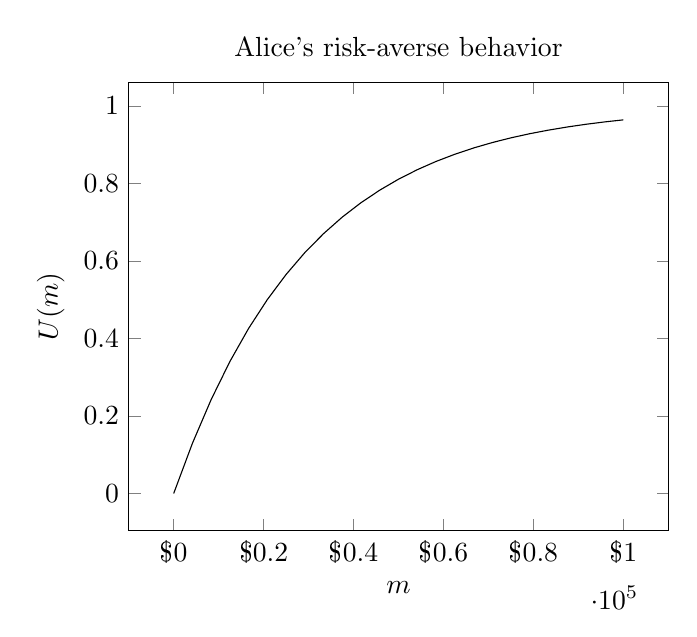
\begin{tikzpicture}
\begin{axis}[
xlabel={$m$},
ylabel={$U(m)$},
xticklabel={\$$\pgfmathprintnumber{\tick}$},
title=Alice's risk-averse behavior,
]
\addplot[domain=0:100000] {1 - exp(-x/30000)};
\end{axis}
\end{tikzpicture}}
\end{minipage}
\hfill
\begin{minipage}{.49\textwidth}
\resizebox{\textwidth}{!}{%
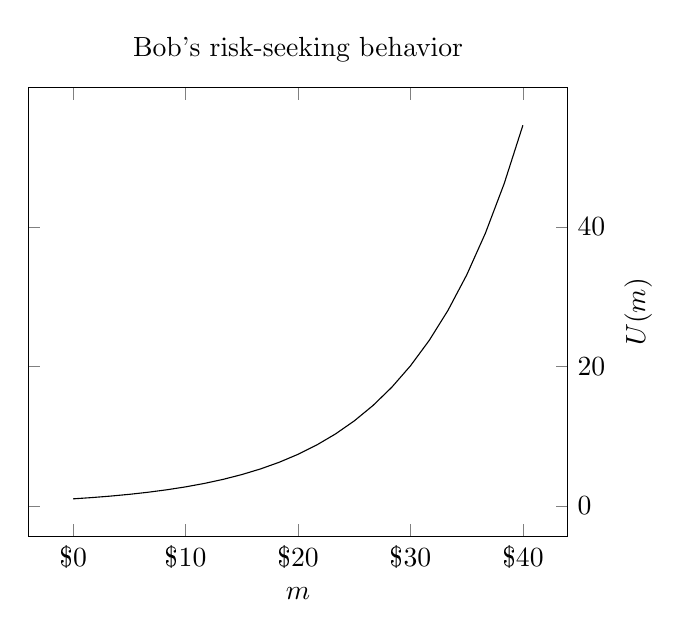
\begin{tikzpicture}
\begin{axis}[
xlabel={$m$},
ylabel={$U(m)$},
xticklabel={\$$\pgfmathprintnumber{\tick}$},
title=Bob's risk-seeking behavior,
yticklabel pos=right,
]
\addplot[domain=0:40] {exp(x/10)};
\end{axis}
\end{tikzpicture}}
\end{minipage}

\end{solution}

\item \emph{Registering for classes.} You are deciding to register for
  one of two classes, IE 5571 or IE 5591. If you register for IE 5571
  you know that you will get a B for sure, but IE 5591 is a lottery
  because the department has not yet decided who will teach the
  class. If Professor England teaches the class then you will get an
  A, but if Professor Doroudi teaches the class then you will get a
  C. You will not know the identity of the instructor until class
  begins and you cannot withdraw from the course once registered. The
  points associated with the letter grades are

\begingroup
\renewcommand{\arraystretch}{1}
\begin{tabular}{cccc}
A&B&C&D \\
4.0 & 3.0 & 2.0 & 1.0
\end{tabular}
\endgroup

Now, you value having fun as much or more than improving your GPA. In
fact, your utility for the points $x$ associated with a letter grade
is $u(x) = \sqrt{x}$. That is to say, your utility for getting a B is
$\sqrt{3}$. The ISyE department head tells you that the probability
that Professor Doroudi will teach IE 5591 is 2/5.

\begin{enumerate}
\item For which class will you register?
\item In general, what is your risk profile toward letter grades?
  (A \emph{brief} answer will suffice.)
\item Your preferences satisfy the conditions of the Expected Utility
  Theorem.  Furthermore, your utility function $u(x)$ was determined
  via questions pertaining to preferences between pairs of
  alternatives (including lotteries). Is it appropriate to say that
  receiving an A is twice as desirable as receiving a D?
\end{enumerate}

\begin{solution}
\bs
The utility of registering for IE 5571 is
\[ u(B) = \sqrt{3} \]
By the expected utility property, the utility of a lottery is its
expected utility. So the utility of registering for IE 5591 is
\begin{align*}
  u\left(L\left(\frac{3}{5},~A,~C\right)\right) &= \frac{3}{5}u(A) + \frac{2}{5}u(C) \\
                  &= \frac{3}{5}\sqrt{4} + \frac{2}{5}\sqrt{2} \\
                  &= \frac{6 + 2\sqrt{2}}{5}
\end{align*}
which is greater than $\sqrt{3}$, so you will register for IE 5591.
In general you are risk-averse with respect to letter grades. It
is \emph{not} appropriate to say that receiving an A is twice
as desirable as receiving a D. Utility functions are defined for
interval scales, not for ratio scales.

\end{solution}

% written by Emily
\item \emph{Preference orderings and utility functions.}  This
  exercise is inspired from discussion in~\cite{resnik:1987}.  Suppose
  you have a goal to be a great long-distance runner.  There are two
  choices involved with this goal in the form of $(x;y)$ where $x$
  represents the number of miles you are able to run in a day after
  you have trained for a month, anywhere from zero to 30 miles, and
  $y$ represents the total number of miles ran to train over the
  course of the month, anywhere from zero to 500. Both $x$ and $y$ are
  continuous distances, and $x \le y$. In general you prefer to be
  able to run farther with less training, but you always prefer to be
  able to run father no matter how much you have to train. For
  example,
  \[
  (x=25~\text{miles}; y=500~\text{miles}) \succ (x=24~\text{miles}; y=200~\text{miles})
  \]
  The symbol `$\succ$' means ``is preferred to''.  Don't confuse that
  symbol with the mathematical inequality symbol `$>$' (although I
  suspect that the resemblence is intended). Note that, as defined, your
  preference ordering satisfies the completeness and transitivity
  properties (see the discussion on page~\pageref{rules-of-consistency}). 
  Is it possible to represent your
  preferences with a single (real-valued) number? That is to say, is
  there a function $u(x,y) : (x,y) \mapsto \mathbb{R}$ with the
  following property
  \[
  (x_1,y_1) \succ (x_2,y_2)~\implies~u(x_1,y_1) > u(x_2,y_2)
  \]
  To make things a little easier, you can restrict $u$ to be a linear
  function of $x$ and $y$. Support your answer with an explanation
  \ldots a formal proof is great, but not required.

\begin{solution}
  \bs I think it is not possible to represent $u$ as a linear
  function of $x$ and $y$. Define $w=500-y$, so that we can represent
  an alternative as $(x,w)$ with the interpretation that more is always
  better, but $x$ still has priority. Now, a linear function will have
  the form
  \[
  u(x,w) = Ax + Bw
  \]
  where $A$ and $B$ are constants.
  It is enough to show a situation where $(x_1;w_1) \succ (x_2;w_2)$
  but that $u(x_1,w_1) < u(x_2,w_2)$. We can write $x_2=x_1-\delta_x$
  and $w_2=w_1+\delta_w$ where $\delta_x > 0$ (so that $x_1>x_2$).
  Now,
  \[
  u(x_1,w_1) = Ax_1 + Bw_1
  \]
  and
  \begin{align*}
    u(x_2,w_2) &= u(x_1-\delta_x,w_1+\delta_w) \\
    &= A(x_1-\delta_x) + B(w_1 + \delta_w) \\
    &= Ax_1 - A\delta_x + Bw_1 + B\delta_w \\
    &= Ax_1 + Bw_1 + (B\delta_w - A\delta_x)
  \end{align*}
  We need only to show that $B\delta_w-A\delta_x > 0$.
  \begin{align*}
    B\delta_w - A\delta_x &> 0 \\
    B\delta_w &> A\delta_x \\
    \frac{\delta_w}{\delta_x} &> \frac{A}{B}
  \end{align*}
  Note that $\delta_w = w_2-w_1 = y_1-y_2 \leq 500$, but because $x$
  is continuous, we can choose $\delta_x$ and $\delta_w$ to satisfy
  the last inequality, which means that $u(x_1,w_1) < u(x_2,w_2)$.
\end{solution}

\end{enumerate}
